\documentclass[10pt,a4paper]{book}
\usepackage[utf8]{inputenc}
\usepackage{amsmath}
\usepackage{amsfonts}
\usepackage{subfig}
\usepackage{amssymb}
\usepackage{epigraph}
\usepackage{makecell}
\usepackage{xcolor}
\usepackage{multirow}
\usepackage{graphicx}
\author{Alberto Rescia}
\newcommand{\code}[1]{\texttt{#1}}

\begin{document}

\chapter{Boosted Xbb tagger}

The higher centre-of-mass energy available in Run 2 necessitated the development of a dedicated boosted tagger to identify b-jets in topologies for which particles such as, but not limited to, the Higgs boson decay to $b$-quarks at a small angular distance from each other. The resulting $b$-jets are contained within a large-R jet of radius $R = 1.0$, and the tagging algorithm is applied directly to this jet. This tagger is known as the \emph{Xbb tagger}.

\section{Introduction to the Xbb tagger}
The Xbb tagger is a neural network trained on the the large-R jet kinematics and on information stemming from VR trackjets used to resolve the individual $b$ hadron decays. 

\code{AntiKt10LCTopoTrimmedPtFrac5SmallR20Jets} are used for training. These jets must have a $p_t$ in the range $250 < p_t < 3000$~GeV and $\vert \eta\vert < 2.0$. VR trackjets with are ghost-associated to the large-R jet. They must have $p_t > 7$~GeV, $\vert \eta \vert < 2.5$ and at least two track constituents. VR trackjets are ghost-associated to the large-R jet. This procedure consists in artificially suppressing their momentum, and re-running the anti-$k_t$ clustering algorithm on all constituents of the large-R jet together with the ``ghost" VR trackjets. If the algorithm finds the ghosts as constituents of the new jet, the VR trackjet is associated.

The probabilities $p_b$, $p_c$ and $p_\text{light}$ from up to three (if available) VR trackjets associated to large-R jet are used to train the Xbb tagger. These are obtained from the DL1r tagging algorithm. The list of input variables is concluded with kinematic information from the large-R jet, specifically the $p_t$ and $\eta$. 

Jets from $H\rightarrow b\bar{b}$, $Z^\prime \rightarrow t\bar{t}$ and multijet samples are used to train the Xbb tagger. In the $H\rightarrow b\bar{b}$ sample, a Higgs boson is required to be ghost-matched to the large-R jet. Large-R jets used for training are downsampled in such a way that the $p_t$ distribution in the three samples is the same. A flat jet mass distribution is also requested to avoid learning the Higgs mass.

The Xbb tagger output is a discriminant which gives the likelihood of the large-R jet coming from a Higgs boson decaying to a pair of b-quarks vs. $t\bar{t}$ or multijet

\begin{equation}
    D_{Xbb} = \ln \left( \frac{p_{\text{Higgs}}}{f_{\text{top}} \cdot p_{\text{top}} + (1 - f_{\text{top}}) \cdot p_{\text{multijet}}} \right)
    \label{eq:dxbb},
\end{equation}
where $f_\text{top} = 0.25$. 

Figure \ref{xbb discriminant} shows the $D_{Xbb}$ output for jets with $p_t > 250$~GeV and mass $76 < m_J/\text{GeV} < 146$ from Higgs, top and multijet samples compared to the output obtained by directly tagging the VR trackjets with DL1r. The additional discrimination power of the dedicated tagger is evident. The Higgs efficiency vs. $t\bar{t}$ and multijet rejection for various values of $f_{\text{top}}$ is instead shown in Figure \ref{fig:xbb_eff}.

\begin{figure}
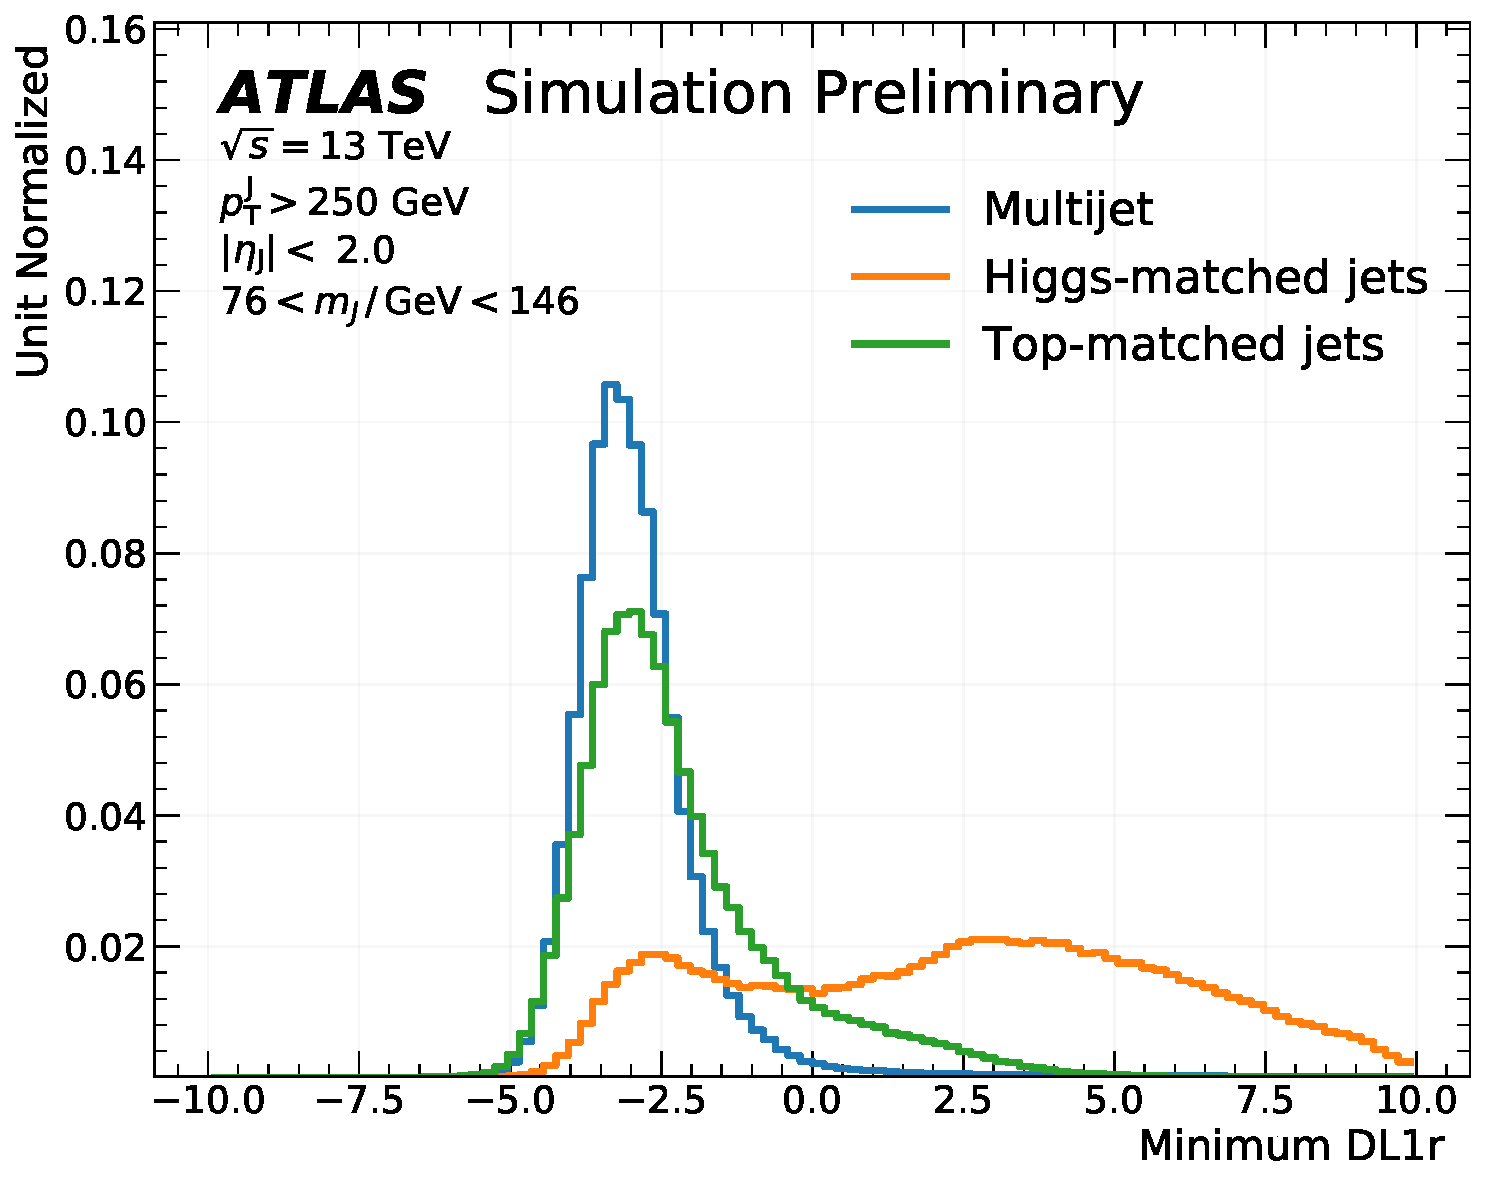
\includegraphics[width=0.485\linewidth]{ftag/xbb_dl1.pdf}
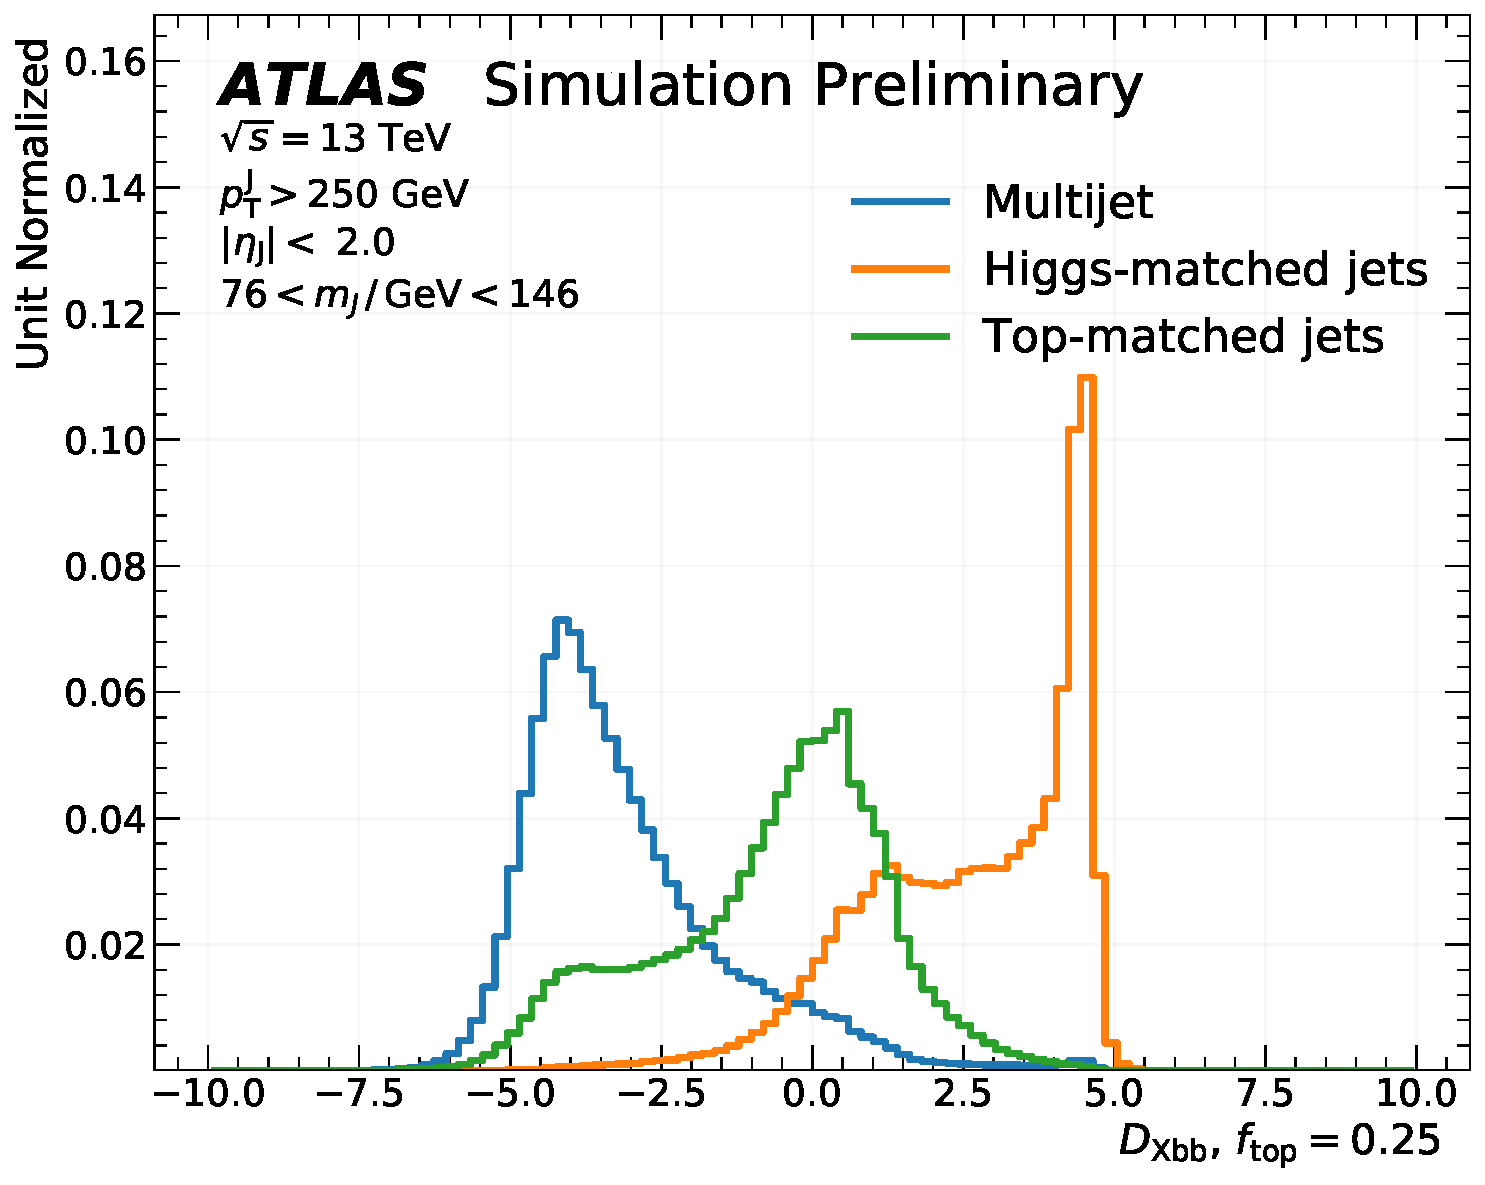
\includegraphics[width=0.485\linewidth]{ftag/xbb.pdf}
\caption{The Xbb discriminant distribution for Higgs, top and multijet samples when both VR trackjets are required to pass a minimum DL1r threshold (left) vs. for the dedicated Xbb tagger (right)\cite{ATLAS:2020ixf}.}
\label{xbb discriminant}
\end{figure}

\begin{figure}
    \centering
    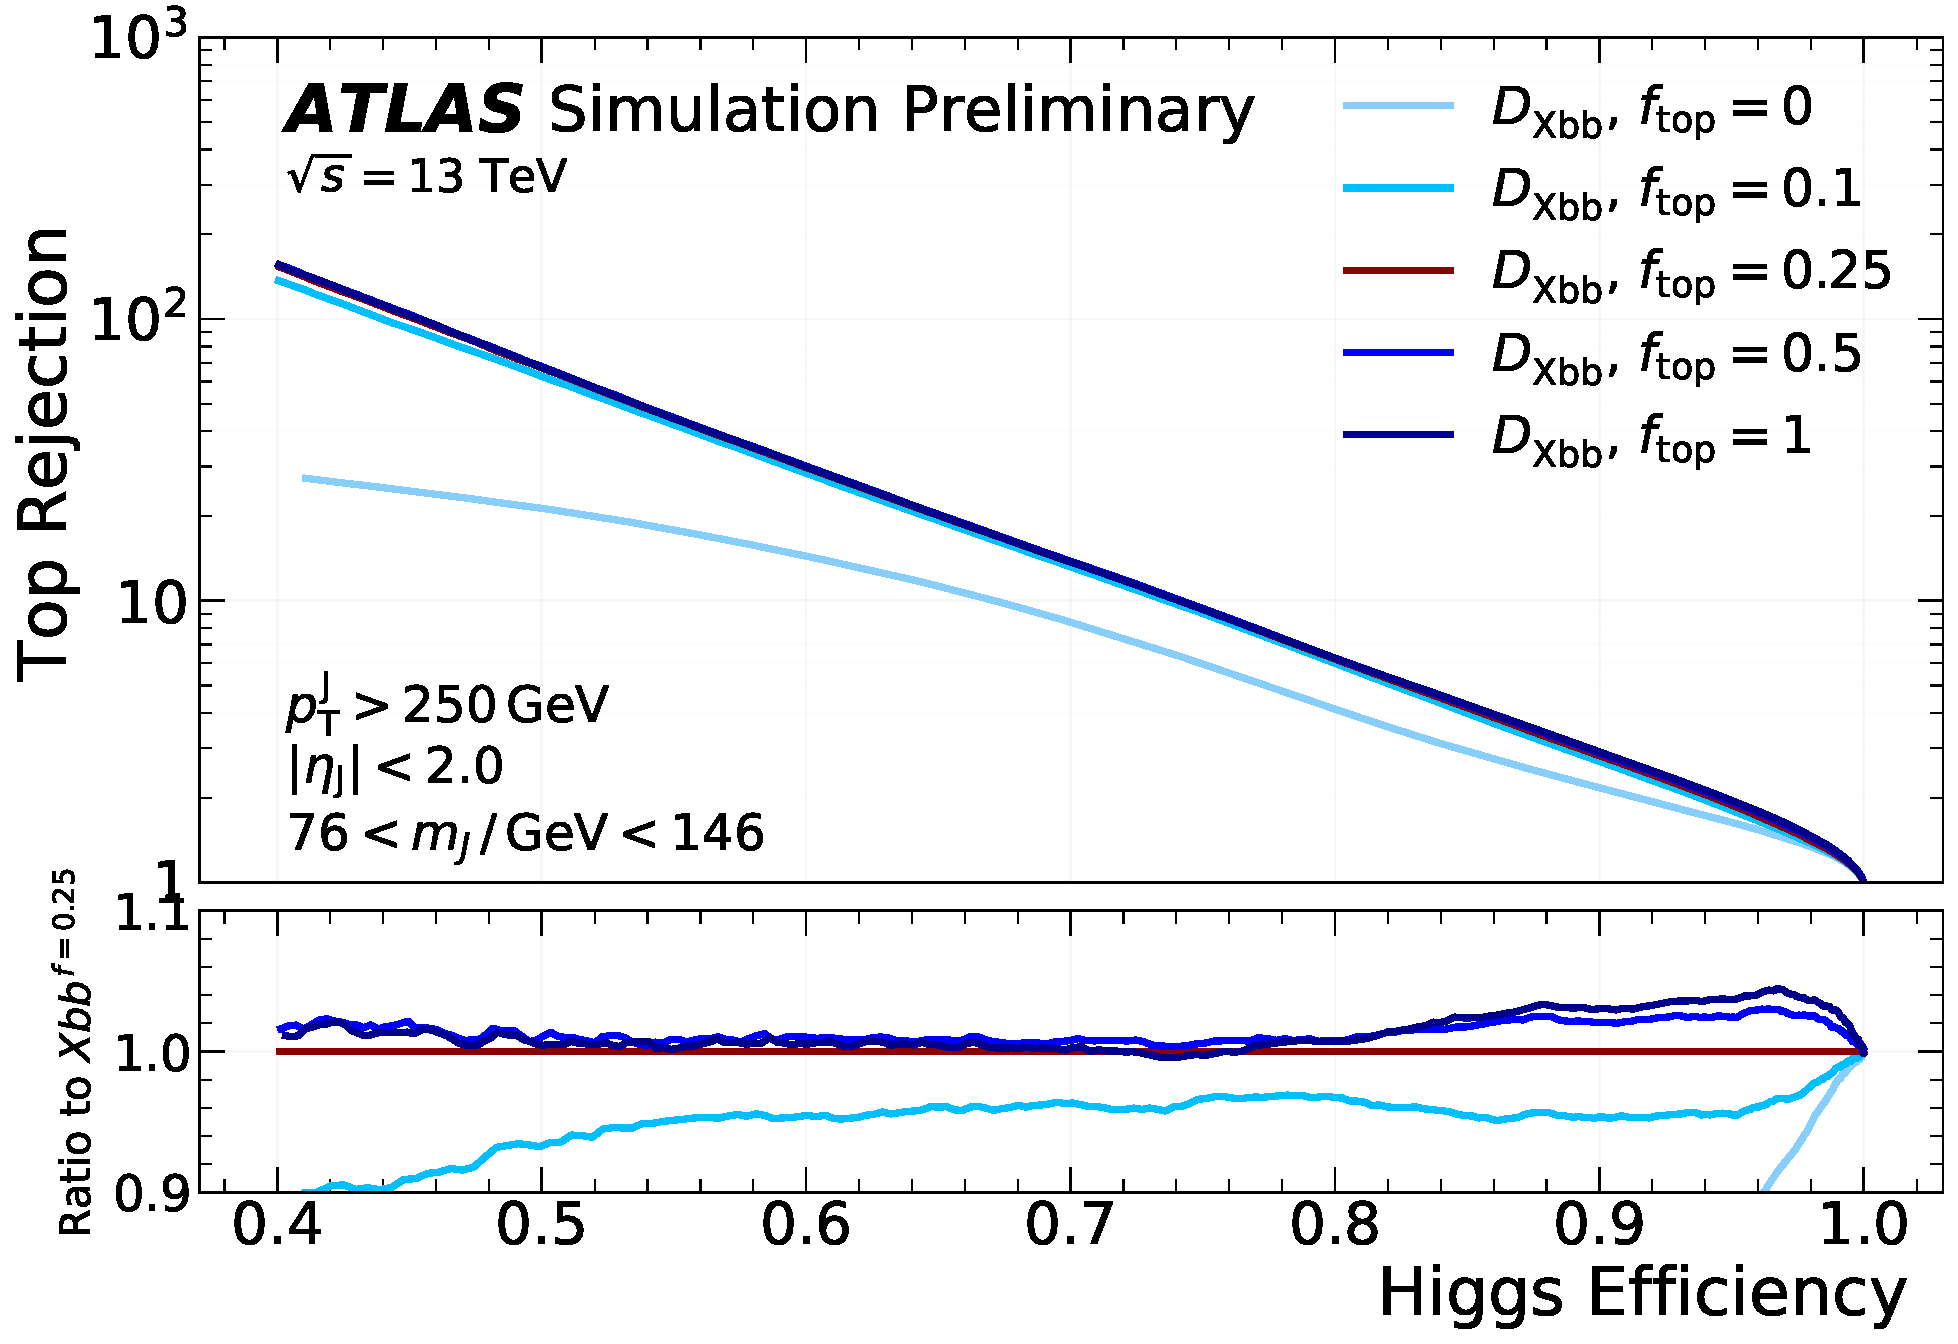
\includegraphics[width=0.485\linewidth]{ftag/xbb_ttbar_eff.pdf}
    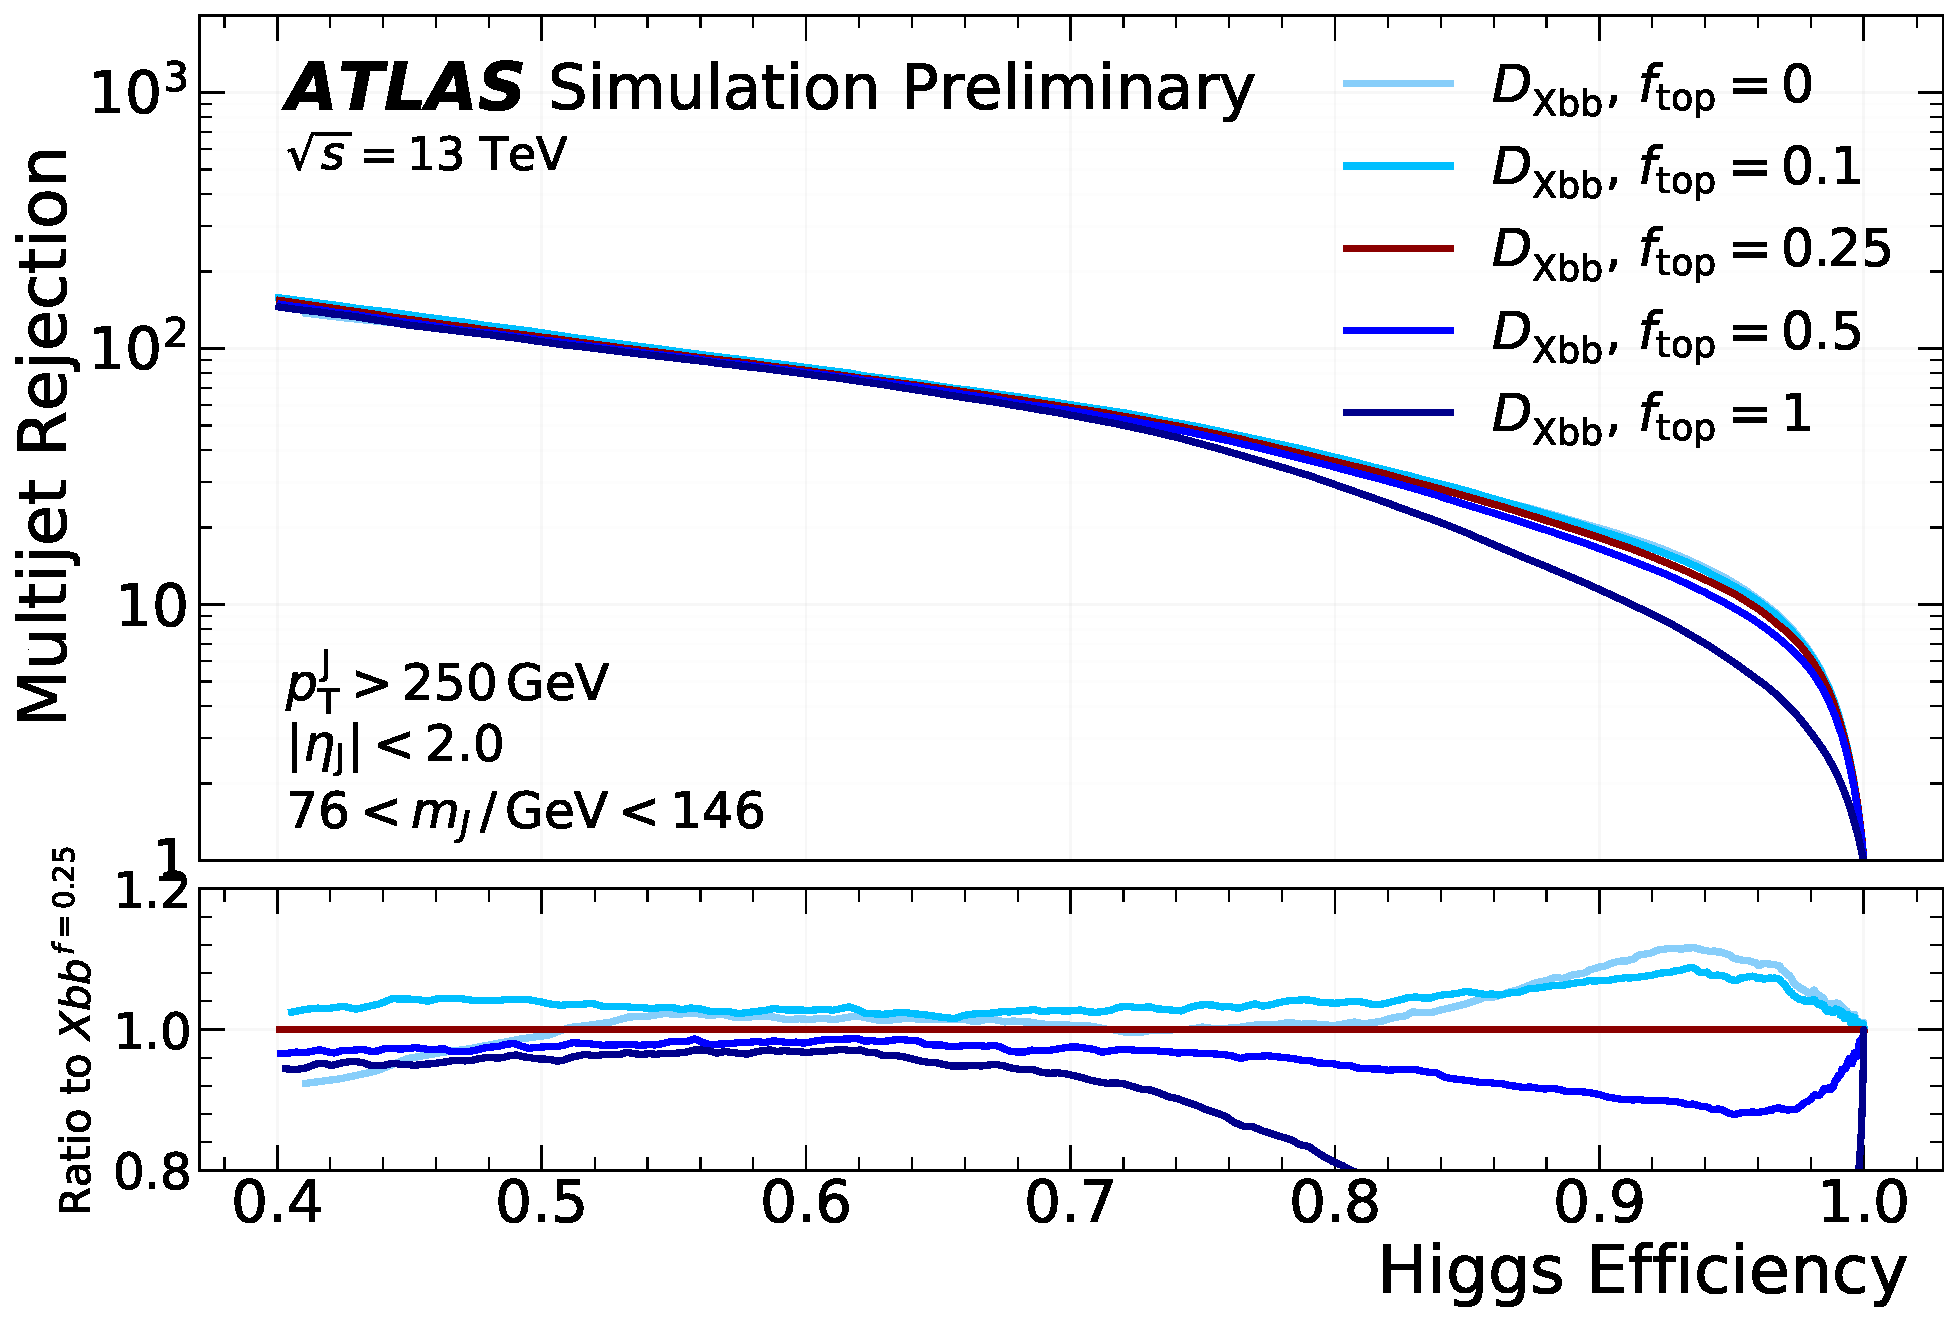
\includegraphics[width=0.485\linewidth]{ftag/xbb_multijet_eff.pdf}
    \caption{The $H\rightarrow b\bar{b}$ tagging efficiency vs. $t\bar{t}$ (left) and multijet (right) rejection~\cite{ATLAS:2021gik}.}
    \label{fig:xbb_eff}
\end{figure}

\section{Calibration}

As the Xbb tagger is trained exclusively on simulated data, it must be calibrated to be used effectively. The calibration ensures that the efficiency of the tagger matches between data and MC. The full Run 2 dataset was used. This calibration constituted my ATLAS Qualification Project.

The calibration was carried out on three final states. The signal efficiency $X\rightarrow b\bar{b}$ is calibrated on $Z (\righarrow b\bar{b}) + \text{jets}$ and $Z(\righarrow b\bar{b})\gamma$ events, while the top and multijet backgrounds are calibrated using $t\bar{t}$ and $g\rightarrow b\bar{b}$ events. My worked focused on the $g\rightarrow b\bar{b}$, and is described below. For details regarding the other calibrations, cfr. Reference~\cite{ATLAS:2021gik}.

\subsection{$g\rightarrow b\bar{b}$ calibration}
\label{gbb}
The calibration focused on dijet events, i.e. $2 \rightarrow 2$ QCD processes. At the MC level, an inclusive sample was simulated along with a sample in which the events are required to contain a muon at truth level. This muon is required to have $p_t > 3$~GeV and $\vert \eta \vert < 2.8$. 

Objects are selected as described above: a large-R jet satisfying the selection criteria of the Xbb tagger is identified, and up to three VR trackjets are ghost-matched to the jet, henceforth referred to as \emph{subjets}. One subjet is required to contain a muon matching the appropriate selection criteria to preferentially favour jets containing heavy flavours. This subjet is known as the \emph{muon jet}. If more than one subjet contains a muon, the one with the highest $p_t$ is called the muon jet.

Subjets are subsequently labelled according to their truth-level flavour content: the label $B$ is assigned if a B hadron is ghost-matched to the subjet, $C$ if a C hadron is ghost-matched, $L$ if no heavy hadrons are ghost-matched, and $x$ if a subjet of that index is not present in the large-R jet.  

The flavour label is used to determine the flavour category of the large-R jet based on its subjets. The MC to data fit is carried out in each flavour category of the large-R jet. As up to three subjets can be considered in each large-R jet, a simplified labelling scheme is applied to the large-R jet. Labels \emph{BB}, \emph{BL}, \emph{CC}, \emph{CL} or \emph{LL} are assigned. The labelling scheme is explained in detail in Table \ref{tab:jet_flavors}.

\begin{table}[h]
\label{tab:jet_flavors}
\centering
\begin{tabular}{|c|c|}
\hline 
\textbf{Large-R jet flavour category} & \textbf{Subjet flavours} \\ 
\hline 
BB & \makecell{BBB, BBC, BBL, BBx,\\ BCB, BLB, CBB, LBB} \\ 
\hline 
BL & \makecell{BCC, BCL, BCx, CBC, CBL, CBx,\\ CCB, BLC, BLL, BLx, LBC, LBL,\\ LBx, CLB, LCB, LLB, Bxx} \\ 
\hline 
CC & CCC, CCL, CCx, CLC, LCC \\ 
\hline 
CL & CLL, CLx, LCL, LCx, LLC, Cxx \\ 
\hline 
LL & LLL, LLx, Lxx \\ 
\hline 
\end{tabular} 
\caption{The large-R Jet flavour categories and corresponding subjet flavours.}
\end{table}

%introduzione xbb tagger
%calibration details - Zbb, gbb, ttbar, flavour fit
%non star lì a mettere plots inutili, ma scrivi esplicitamente che hai partecipato alla calibrazione
\subsection{Fit strategy}

After labelling the large-R jet, a template of a flavour-sensitive observable is made for fitting MC to data. For this calibration, the mean $S_{d0}$ was chosen, where the mean is calculated on the three highest $p_t$ tracks associated to the jet. The average is specifically chosen to reduce the influence of outliers in light-flavour jets, such as mismodelled tracks or $K_s$ decays.

Four regions/jets are considered for the template fit: the muon jet and the leading non-muon jet, for a double-b-tagged (with DL1r) and non-double-b-tagged large-R jet. A 60\% b-tagging working point is chosen. The fit is carried out in several different $p_t$ regions of the large-R jet: below 280~GeV, 280-310~GeV, 310-340~GeV, 340-380~GeV, 380-420~GeV, 420-460~GeV, 460-500~GeV, 500-550~GeV, 550-600~GeV, 600-750~GeV, 750-1000~GeV, and above 1000~GeV.

A smoothing procedure is applied in order to reduce statistical fluctuations which may impede the convergence of the fit. This is achieved by merging bins in which these fluctuations are present. Bins are merged when the statistical uncertainty is greater than the systematic uncertainty. 

For a given bin with nominal entries $N$ and systematic variation $S$, with relative errors $\delta N$ and $\delta S$, the total error is given by $\delta M = \sqrt{\delta S^2 + \delta N^2}$, for uncorrelated variations, or $\delta M = \max(\delta N, \delta S)$ for correlated variations. If for a bin $\vert S  - N\vert < \delta M$, this bin is merged with the neighbouring bin with the highest value of $\delta M/M$. This is the rebinning step in the template definition.

To further reduce the statistical fluctuations of the systematic variations, for each pair of neighbouring bins $b_j$ and $b_{j-1}$ the value
\begin{equation}
    X_{j-1,j} = \left| \frac{S_j - N_j}{N_j} - \frac{S_{j-1} - N_{j-1}}{N_{j-1}} \right|
\end{equation}
and relative error
\begin{equation}
\delta X_{j-1,j} = \sqrt{\frac{\delta M_j^2}{N_j^2} + \frac{\delta M_{j-1}^2}{N_{j-1}^2}}
\end{equation}
is calculated. If for some pair $\delta X < X$, the bins in the pair are merged. The systematic variations calculated in the merged bin, and propagated back to the original binning. The end result is an ease of tension in the fit. 

The fit method chosen is a binned profile likelihood. In each histogram bin $i$, the expectation value for the number of entries $E[n_i]$ is given by 
\begin{equation}
    E[n_i] = \prod_{xx} f_{xx} y_{xx,i} = \vec{f} \cdot \vec{y_i},
\end{equation}
where $y_{xx,i}$ is the nominal number of entries in the bin and $f_{xx}$ is a correction factor applied to the flavour template $xx$. The template distributions depend on nuisance parameters (NPs) $\vec{\theta}$ with prior probability distributions determined from auxiliary measurements. The priors are assumed to follow a split-normal distribution $\mathcal{SN}$ with a width on each side given by a variation histogram. The likelihood function for the overall number of entries in each bin and in each template is thus given by
% Requires: \usepackage{amsmath}
\begin{equation}
    \mathcal{L}(\vec{f}, \vec{\theta}) = \prod_{i=1}^{N} e^{-(\vec{f} \cdot \vec{y}_i)} \frac{(\vec{f} \cdot \vec{y}_i)^{n_i}}{n_i!} \prod_{k} \mathcal{SN}(\theta_k),
    \label{eq:placeholder}
\end{equation}
where the vector of NPs is taken to be of length $k$. NPs are taken to be systematic uncertainties, such as modelling uncertainties and those related to the detector reconstruction.

The fit in the tagged and anti-tagged regions is simultaneous. The regions are independent, so it is sufficient to multiply the likelihoods relative to each region to obtain the full likelihood.

Maximising the likelihood corresponds to extracting the best-fit value of $\vec{f}$, which corresponds to the measuring the flavour contribution in each template. The four tag regions are fit simultaneously, though the fit in each of the eight large-R jet $p_t$ slices is independent. The scale factor and flavour corrections are allowed to float freely, and are extracted from the fit.

Figure \ref{fig:prefit} shows the pre-fit templates in the four regions considered for the fit, for the large-R jet $p_t$ slice between 600-750~GeV. 

The post-fit agreement is shown in Figure \ref{fig:postfit}. 

The scale factors extracted from the fit in each $p_t$ slice are shown in Figure \ref{fig:sf_sd0}. They are entirely below unity, indicating a higher cross section predicted than that actually measured. As indicated by the small uncertainties on the scale factor, some $p_t$ bins are also highly constrained. This may be caused by irregular shape variations and statistical fluctuations in the template which lead to a reduction of flexibility in the fit procedure.

\begin{figure}
    \centering
    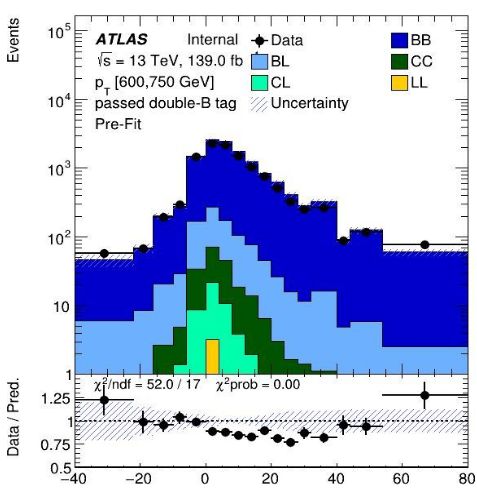
\includegraphics[width=0.485\linewidth]{ftag/prefit_600-750_sd0/muon_pass.png}
    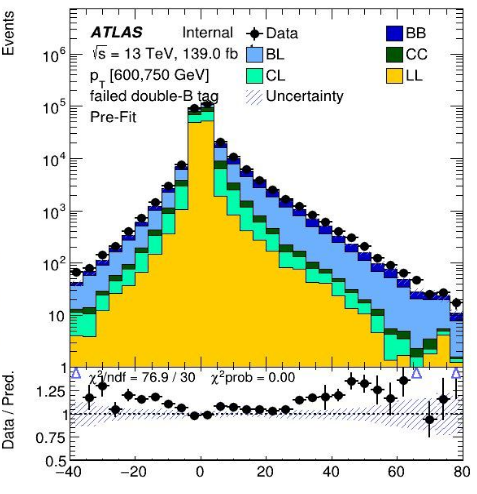
\includegraphics[width=0.485\linewidth]{ftag/prefit_600-750_sd0/muon_fail.png} \\
     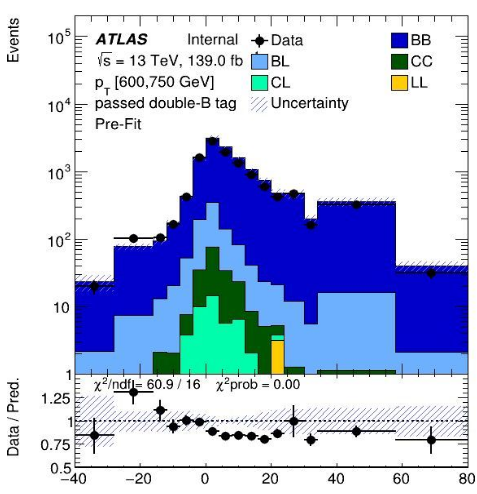
\includegraphics[width=0.485\linewidth]{ftag/prefit_600-750_sd0/nonmuon_pass.png}
    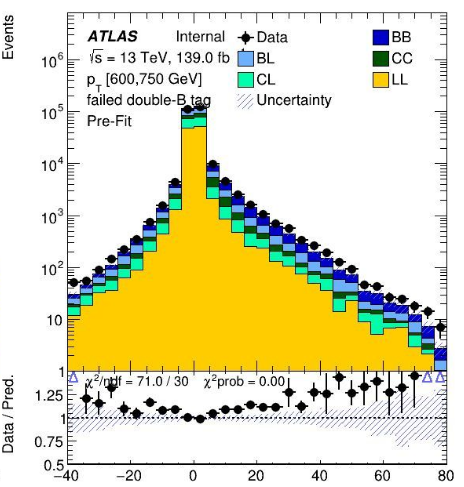
\includegraphics[width=0.485\linewidth]{ftag/prefit_600-750_sd0/nonmuon_fail.png} \\
    \caption{The pre-fit agreement in the four templates used for the $g\rightarrow b \bar{b}$ calibration. The top row corresponds to the muon jet and the bottom row to the leading non-muon jet. The left column shows the double-b tagged large-R jet and the right column the anti-tagged jet.}
    \label{fig:prefit}
\end{figure}

\begin{figure}
    \centering
    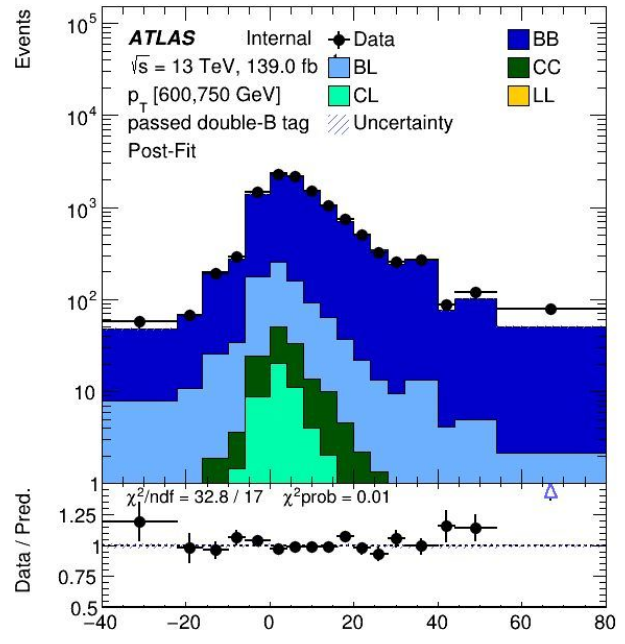
\includegraphics[width=0.485\linewidth]{ftag/postfit_600-750_sd0/muon_pass.png}
    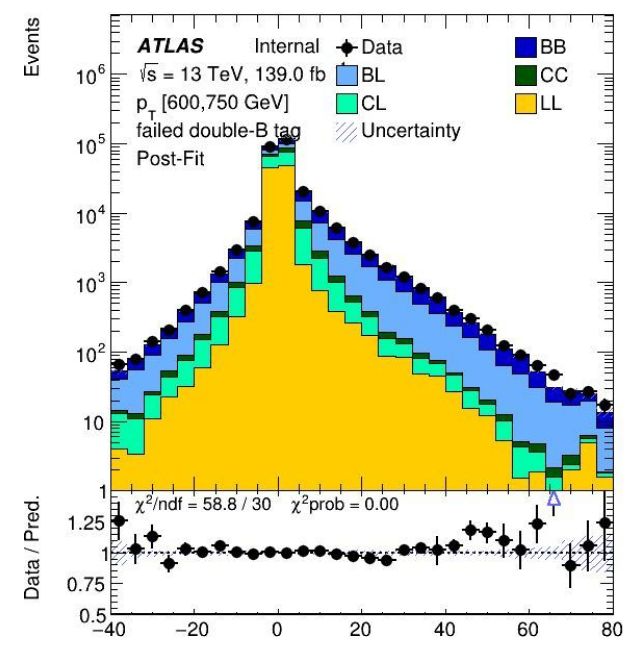
\includegraphics[width=0.485\linewidth]{ftag/postfit_600-750_sd0/muon_fail.png} \\
     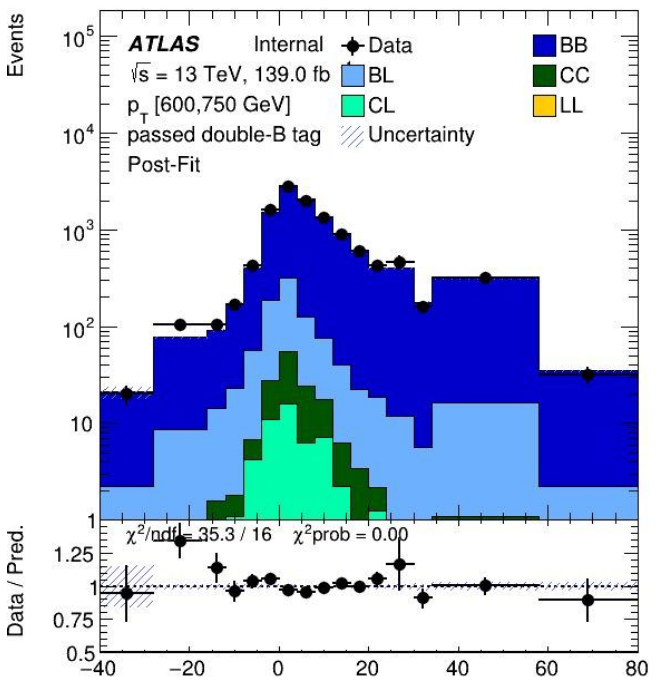
\includegraphics[width=0.485\linewidth]{ftag/postfit_600-750_sd0/nonmuon_pass.png}
    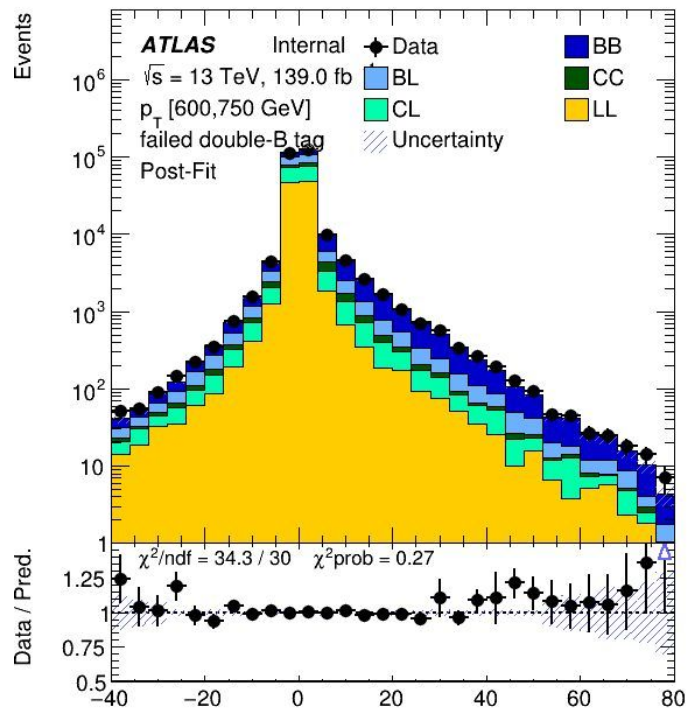
\includegraphics[width=0.485\linewidth]{ftag/postfit_600-750_sd0/nonmuon_fail.png} \\
    \caption{The post-fit agreement in the four templates used for the $g\rightarrow b \bar{b}$ calibration. The top row corresponds to the muon jet and the bottom row to the leading non-muon jet. The left column shows the double-b tagged large-R jet and the right column the anti-tagged jet.}
    \label{fig:postfit}
\end{figure}

\begin{figure}
    \centering
    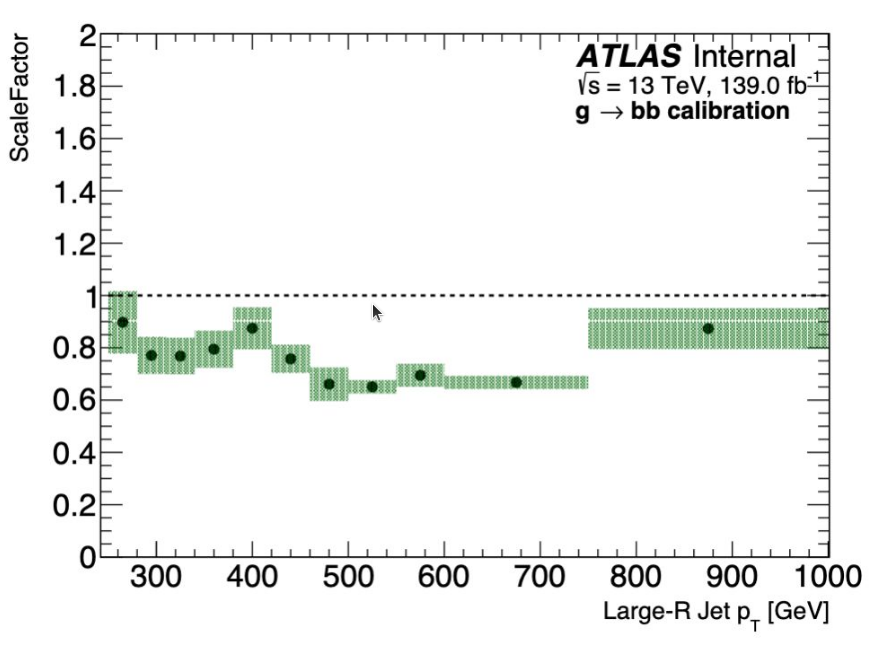
\includegraphics[width=0.9\linewidth]{ftag/sf_sd0.png}
    \caption{The scale factors in each $p_t$ sliced extracted from the $g\rightarrow b\bar{b}$ fit.}
    \label{fig:sf_sd0}
\end{figure}

\subsection{Systematic uncertainties}

A number of systematic uncertainties come into play when fitting the MC simulation to data. These uncertainties also represent NPs for the fit.

Uncertainties fall within three main categories: experimental uncertainties related to the reconstruction of objects used for the selection, such as jets, tracks, and muons; theoretical uncertainties related to MC modelling; and uncertainties specific to the $g\rightarrow b\bar{b}$ calibration. These include uncertainties on the fragmentation of different species of B hadrons which different lifetimes or on processes that produce tracks with large values of $S_{d_0}$, such as the production of $K_s$ or $\Lambda$.

Besides the systematic uncertainties, extrapolation uncertainties are also considered as NPs. These are applied directly to the scale factors derived from the fit, and account for the fact that the $g\rightarrow b\bar{b}$ calibration explicitly requires a muon jet, which is not a general requirement for users of the Xbb tagger. It also accounts for the fact that the Xbb tagger is meant to be used in cases of $b\bar{b}$ resonances \emph{of any origin}. There are some differences, for instance, between $g\rightarrow b\bar{b}$, $H\rightarrow b\bar{b}$ in terms of angular separation of the jets and colour connection which must be considered. These extrapolation uncertainties are derived from the inclusive MC sample.

The categorisation of systematics is illustrated in full in Table~\ref{tab:uncertainties_cat}. A full list of systematics considered, and whether they are applied exclusively to is available in Table~\ref{tab:uncertainties}. This table also states whether a given systematic is applied to template shape, normalisation, or both. 

% Requires: \usepackage{graphicx}
\begin{table}[hbtp]
    \centering
    \begin{tabular}{|l|p{8.5cm}|}
        \hline
        \textbf{Systematic Uncertainty} & \textbf{Brief Description} \\
        \hline
        \multicolumn{2}{|c|}{\textbf{Template Uncertainties}} \\
        \hline
        'Fake' secondary vertex & Uncertainty on the rate of processes which create large $d_0$ tracks in light-flavour jets. \\
        \hline
        'Fake' muons & Uncertainty on the rate of false-positive muon identification in $b$-jets. \\
        \hline
        $b$-hadron fractions & Uncertainty on the relative production rate of $b$-hadron species. Uncertainty in the inclusive phase-space from the muon requirement used to derive scale factors. \\
        \hline
        $g \rightarrow b \bar{b} \rightarrow X \rightarrow b \bar{b}$ & Uncertainty on extrapolating from $g \rightarrow b \bar{b}$ decays to the general $X \rightarrow b \bar{b}$ case. \\
        \hline
        \multicolumn{2}{|c|}{\textbf{Experimental Uncertainties}} \\
        \hline
        Luminosity & Uncertainty on the full Run 2 integrated luminosity, as measured by the LUCID-2 detector. \\
        \hline
        Pileup Reweighting & Uncertainties on pile-up conditions are applied when reweighting simulations to match data. \\
        \hline
        Jet Energy Scale (JES) & Uncertainty on the reconstruction of large-$R$ jet energies from detector inputs. Applied as 30 independent NPs. \\
        \hline
        Jet Energy Resolution (JER) & Uncertainty on the precision of jet energy reconstruction. \\
        \hline
        Jet Mass Scale (JMS) & Uncertainty on jet mass reconstruction. Calculated separately from JES and applied as 6 independent NPs. \\
        \hline
        Jet Mass Resolution (JMR) & Uncertainty on the precision of jet mass reconstruction. Separate NPs used for Higgs jets and top jets. \\
        \hline
        Muon Reconstruction Efficiency & Uncertainties on the muon reconstruction efficiency and track-to-vertex association \cite{ATLAS:2016lqx}. \\
        \hline
        Muon Momentum Scale & Uncertainty on muon momentum reconstruction \cite{ATLAS:2016lqx}. Includes separate uncertainties on the resolution of ID and MS tracks. \\
        \hline
        Sagitta Bias Correction & Uncertainties due to charge-dependent effects of detector misalignment \cite{ATLAS:2016lqx}. \\
        \hline
        Track reconstruction efficiency & Uncertainties on passive material in the ID and on the GEANT4 model used in simulation. \\
        \hline
        Track fake rate & Uncertainty on the rate of combinatorial fake tracks from large numbers of hits in the ID. \\
        \hline
        Track impact parameter resolution & Uncertainties based on the difference in $d_0$ and $z_0$ resolution between data and MC. \\
        \hline
        \multicolumn{2}{|c|}{\textbf{Theoretical Uncertainties}} \\
        \hline
        Parton Shower & Uncertainty in the parton shower model is measured by comparing PYTHIA 8 and HERWIG 7. \\
        \hline
        Renormalisation Scale & Uncertainties in renormalisation and factorization scales, and in final state radiation (FSR) are assessed by sample weight variations in PYTHIA 8. \\
        \hline
    \end{tabular}
    \caption{Uncertainties on the derivation of $b$-tagging scale factors for the $g\rightarrow b\bar{b}$ calibration of the Xbb tagger.}
    \label{tab:uncertainties_cat}
\end{table}

% Requires: \usepackage{graphicx}
\begin{table}[hbtp]
    \centering
    \begin{tabular}{|l|l|l|}
        \hline
        \textbf{Name} & \textbf{Regions/Templates} & \textbf{Norm/Shape} \\ \hline
        JET\_EffectiveNP\_R10\_GrestTerm & all templates, fully correlated & shape only \\ \hline
        JET\_EtaIntercalib\_Modelling & all templates, fully correlated & shape only \\ \hline
        JET\_EtaIntercalib\_NonClosure\_2018data & all templates, fully correlated & shape only \\ \hline
        JET\_EtaIntercalib\_R10\_TotalStat & all templates, fully correlated & shape only \\ \hline
        JET\_EffectiveNP\_R10\_Pi4 & all templates, fully correlated & shape only \\ \hline
        JET\_EffectiveNP\_R10\_2 & all templates, fully correlated & shape only \\ \hline
        JET\_EffectiveNP\_R10\_3 & all templates, fully correlated & shape only \\ \hline
        JET\_EffectiveNP\_R10\_4 & all templates, fully correlated & shape only \\ \hline
        JET\_EffectiveNP\_R10\_5 & all templates, fully correlated & shape only \\ \hline
        JET\_Flavor\_Composition & all templates, fully correlated & shape only \\ \hline
        MUON\_ID & all templates, fully correlated & shape only \\ \hline
        MUON\_SAGITTA\_RESBIAS & all templates, fully correlated & shape only \\ \hline
        MUON\_SCALE & all templates, fully correlated & shape only \\ \hline
        MUON\_EFF\_TTVA\_SYS & all templates, fully correlated & shape only \\ \hline
        TRK\_RES\_P2\_MEAS & all templates, fully correlated & shape only \\ \hline
        TRK\_RES\_P2\_ERR & all templates, fully correlated & shape only \\ \hline
        TRK\_RES\_D0\_DEAD & all templates, fully correlated & shape only \\ \hline
        TRK\_RES\_Z0\_DEAD & all templates, fully correlated & shape only \\ \hline
        TRK\_EFF\_LOOSE\_GLOBAL & all templates, fully correlated & shape only \\ \hline
        TRK\_EFF\_LOOSE\_T1 & all templates, fully correlated & shape only \\ \hline
        TRK\_EFF\_LOOSE\_PHYSMODEL & all templates, fully correlated & shape only \\ \hline
        TRK\_EFF\_LOOSE\_PP0 & all templates, fully correlated & shape only \\ \hline
        TRK\_FAKE\_RATE\_LOOSE\_PP0 & all templates, fully correlated & shape only \\ \hline
        TRK\_EFF\_LOOSE\_TIDE & all templates, fully correlated & shape only \\ \hline
        TRK\_FAKE\_RATE\_LOOSE\_TIDE & all templates, fully correlated & shape only \\ \hline
        \hline
        Conversion & all templates, fully correlated & normalisation \\ \hline
        HadMat & all templates, fully correlated & normalisation \\ \hline
        LightLongLived & \makecell{electrons/taus flavour categories,\\ only for BB and BL} & normalisation \\ \hline
        BHAD & all templates, fully correlated & shape only \\ \hline
        isr\_muRfac\_65\_\_fsr\_muRfac\_1 & all templates, fully correlated & shape only \\ \hline
        isr\_muRfac\_1\_\_fsr\_muRfac\_0925 & all templates, fully correlated & shape only \\ \hline
        isr\_muRfac\_2\_\_fsr\_muRfac\_1 & all templates, fully correlated & shape only \\ \hline
        isr\_muRfac\_1\_\_fsr\_muRfac\_2 & all templates, fully correlated & shape only \\ \hline
        Herwig & \makecell{merging categories, flavours,\\ only for BB and BL} & shape only \\ \hline
    \end{tabular}
    \caption{Names of the uncertainties included in the final template fit with the correspondent values and usage.}
    \label{tab:uncertainties}
\end{table}

Figure \ref{fig:pulls} shows the pulls derived from the NPs in the template fit, in the $p_t$ bin 600-750~GeV. These are defined as the difference between the postfit ($\hat{\theta}$) and prefit ($\theta_0$) values of a quantity in units of standard deviation $\Delta \theta$
\begin{equation}
    \text{pull} = \frac{\hat{\theta} - \theta_0}{\Delta \theta}.
\end{equation}

From the plot, the systematics with the most significant pulls are those related to the MC uncertainties on the definitions of the individual flavour templates. Some individual systematics related to the fake rate of tracks, initial/final state radiation, and jet modelling compose of the rest of the main contribution.

The correlation matrix of the NPs is also shown in Figure~\ref{correlation}. As can be seen, the most highly correlated NPs are those related the major systematics described above and the normalisation factors of the various flavour templates used for the fit. 

\begin{figure}
    \centering
    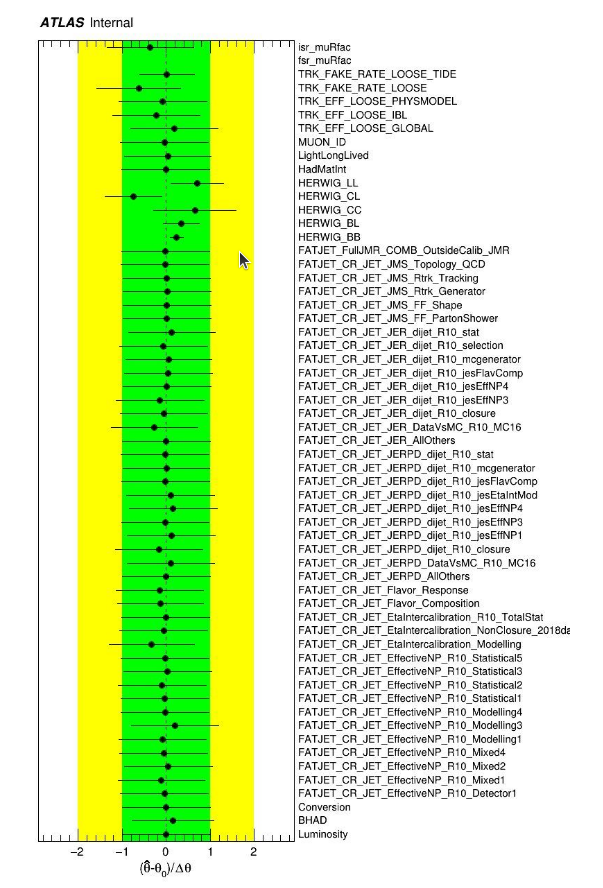
\includegraphics[width=0.8\linewidth]{ftag/pulls_smooth.png}
    \caption{The pulls of the systematic variations affecting the template fit, in the large-R jet $p_t$ region between $600 < p_t/\text{GeV} < 750$.}
    \label{fig:pulls}
\end{figure}

\begin{figure}
    \centering
    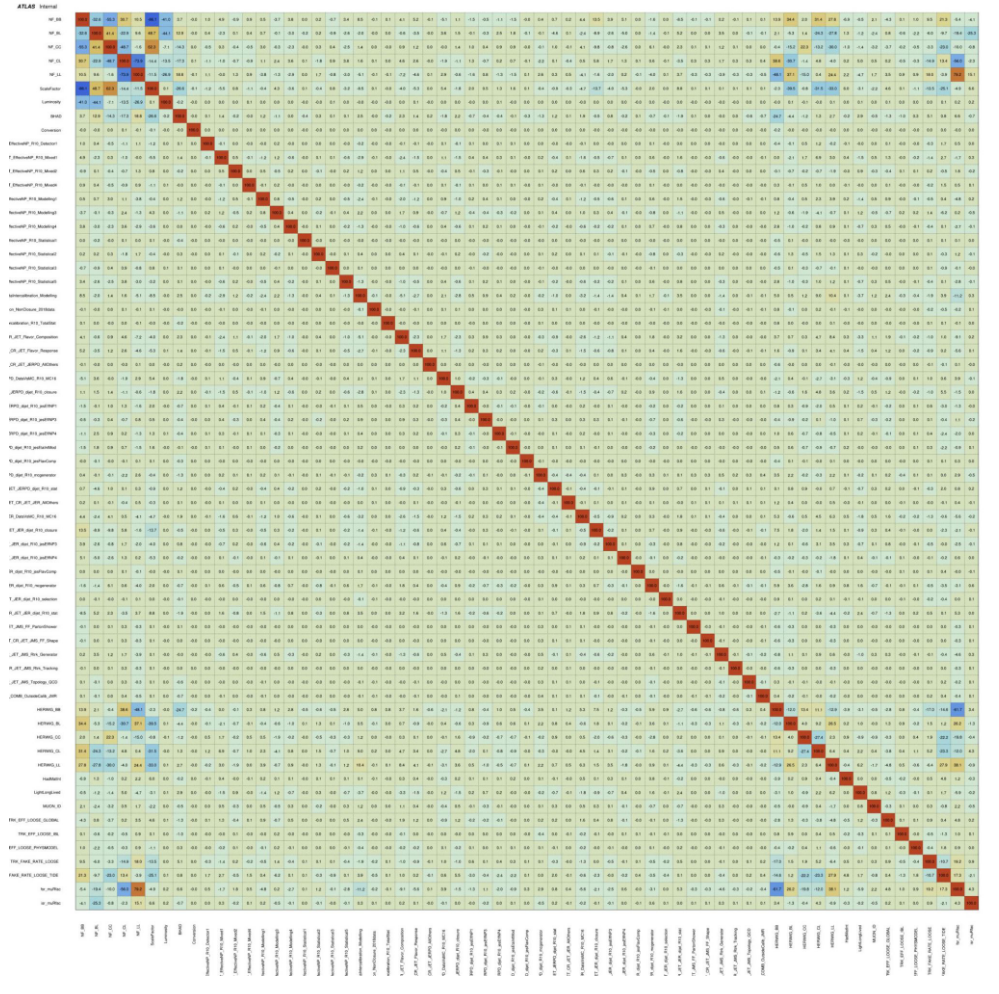
\includegraphics[width=0.8\linewidth]{ftag/np_corr.png}
    \caption{The correlation matrix of the NPs from the template fit, in the large-R jet $p_t$ region between $600 < p_t/\text{GeV} < 750$.}
    \label{fig:correlation}
\end{figure}

\subsection{SV1 Mass Fit}
\label{sv1 fit}

It is also possible to run the fit with a different flavour-sensitive template variable to check the compatibility of the results with the two methods. This was also done, and the secondary vertex (SV1) mass was chosen as the variable used to define the templates.

The SV1 mass corresponds to the mass of the tracks coming from the secondary vertex, as found by the vertex finder described in Section~\ref{SV1}. To reiterate, if it were possible to associate all particles coming from a heavy hadron decay to the secondary vertex, this would be found to have a mass corresponding to that of the heavy hadron, of the order of 5~GeV for $b$ hadrons. In practice, only charged particles can be associated to the secondary vertex, and there is always the possibility of fake tracks and inefficiencies, so the reconstructed vertex tends to have values below 5~GeV. 

Aside from the choice of variable, the details of the fit are otherwise identical. We will thus limit ourselves to the results, with relevant comments when necessary.

In Figures \ref{fig:prefit_sv1} and \ref{fig:postfit_sv1}, we see the prefit and postfit plot for the templates defined with the SV1 mass variable. As compared to the mean $s_{d_0}$, we can see how the SV1 mass distribution is overall smoother, missing the significant peak centred at 0 which was present in the $s_{d_0}$. Some flavour templates, particularly LL in the non-muon jet in the fail region, do portray peaks, however.

\begin{figure}
    \centering
    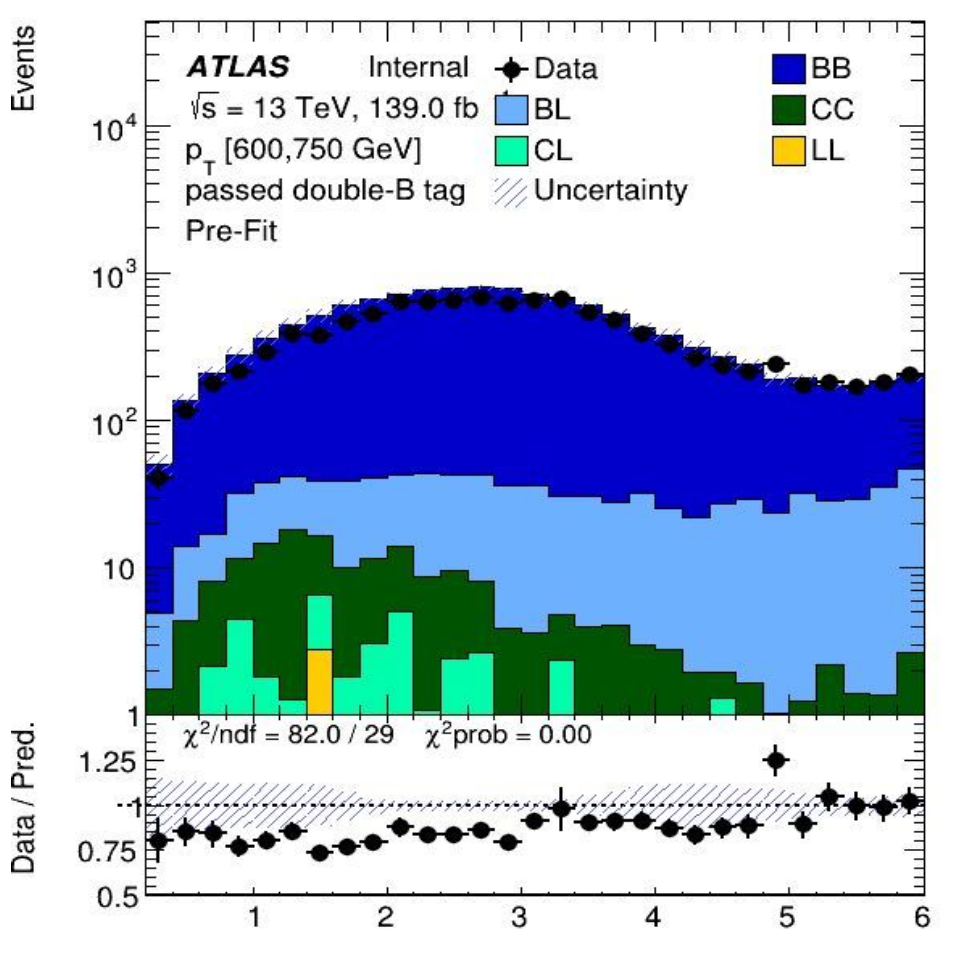
\includegraphics[width=0.485\linewidth]{ftag/sv1Fit/prefit/muon_pass.png}
    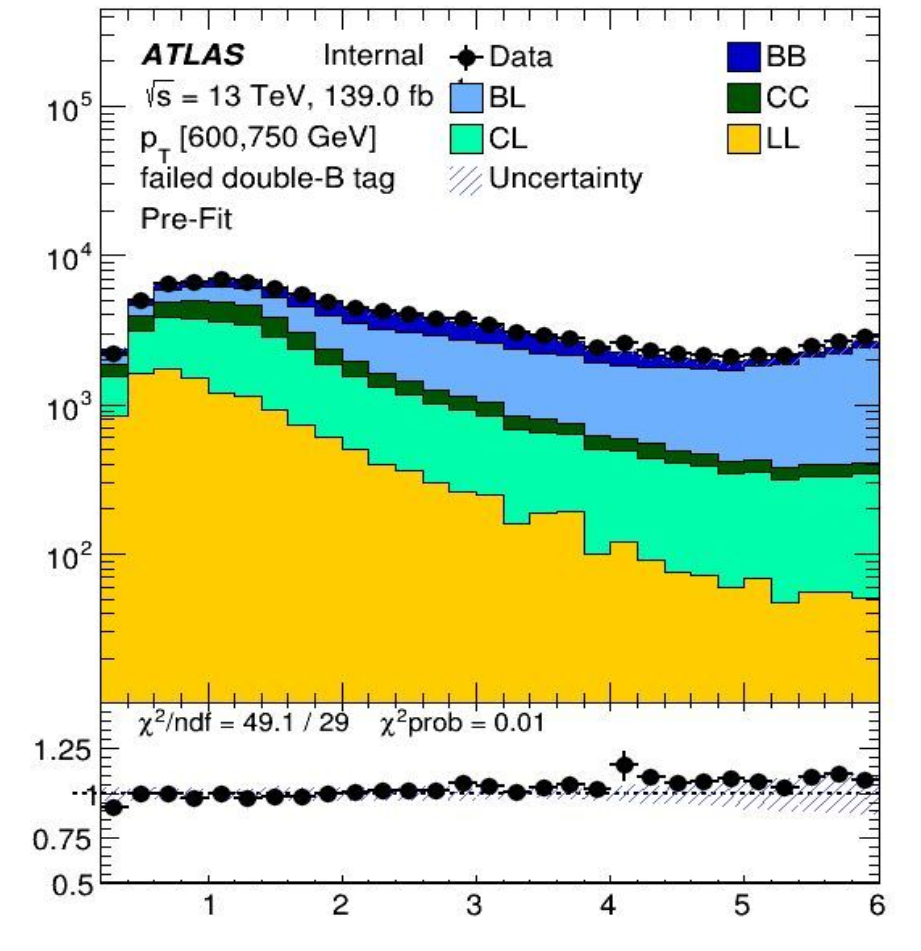
\includegraphics[width=0.485\linewidth]{ftag/sv1Fit/prefit/muon_fail.png} \\
     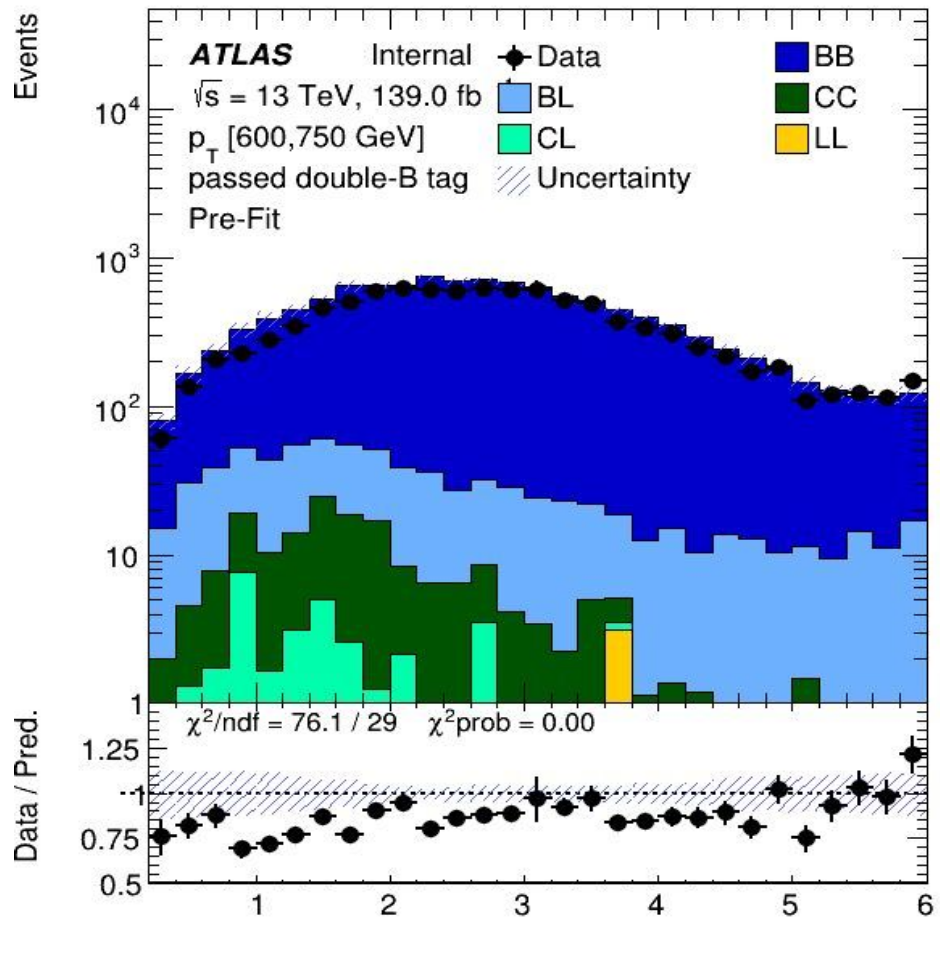
\includegraphics[width=0.485\linewidth]{ftag/sv1Fit/prefit/nonmuon_pass.png}
    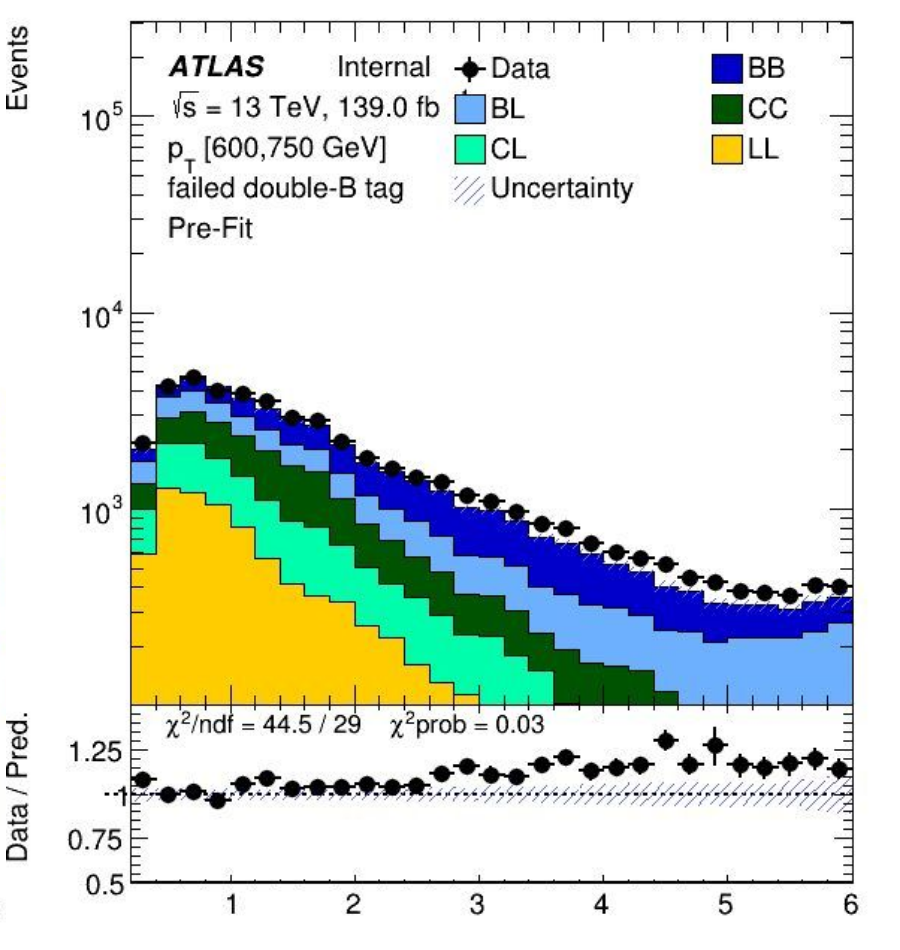
\includegraphics[width=0.485\linewidth]{ftag/sv1Fit/prefit/nonmuon_fail.png} \\
    \caption{The pre-fit agreement in the four templates used for the $g\rightarrow b \bar{b}$ calibration with the SV1 mass variable. The top row corresponds to the muon jet and the bottom row to the leading non-muon jet. The left column shows the double-b tagged large-R jet and the right column the anti-tagged jet.}
    \label{fig:prefit_sv1}
\end{figure}

\begin{figure}
    \centering
    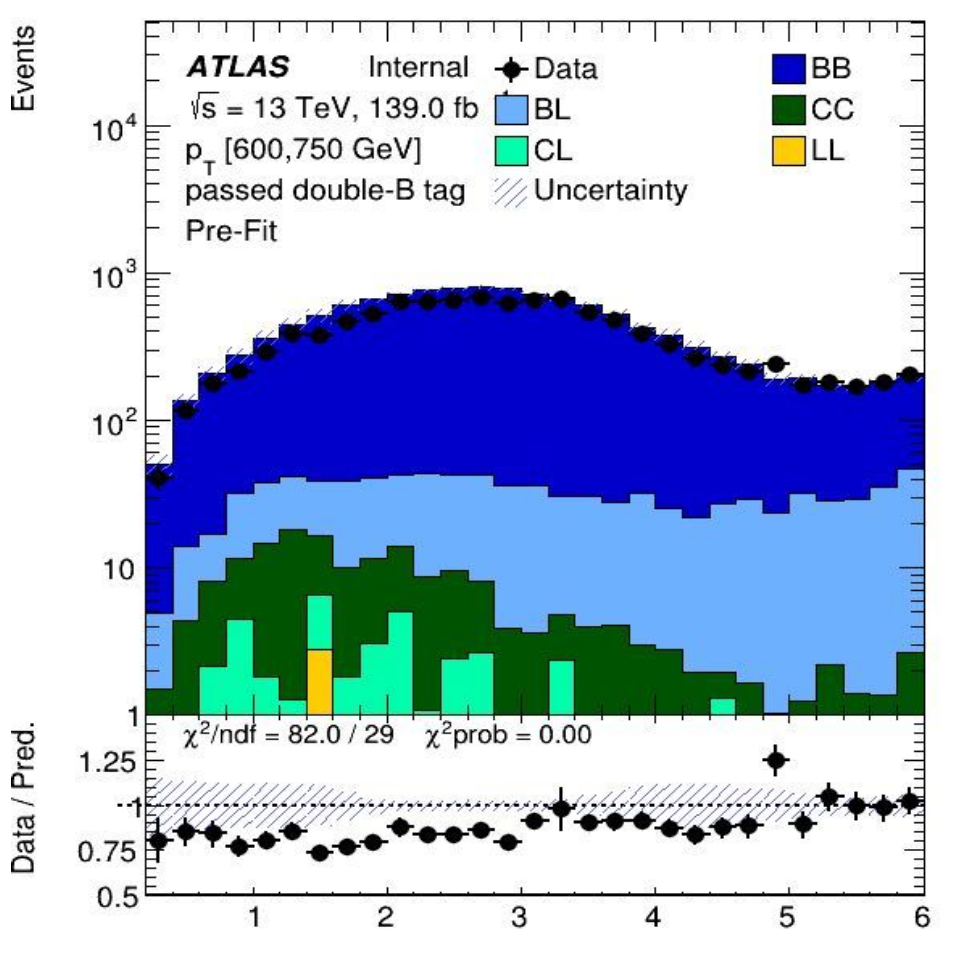
\includegraphics[width=0.485\linewidth]{ftag/sv1Fit/prefit/muon_pass.png}
    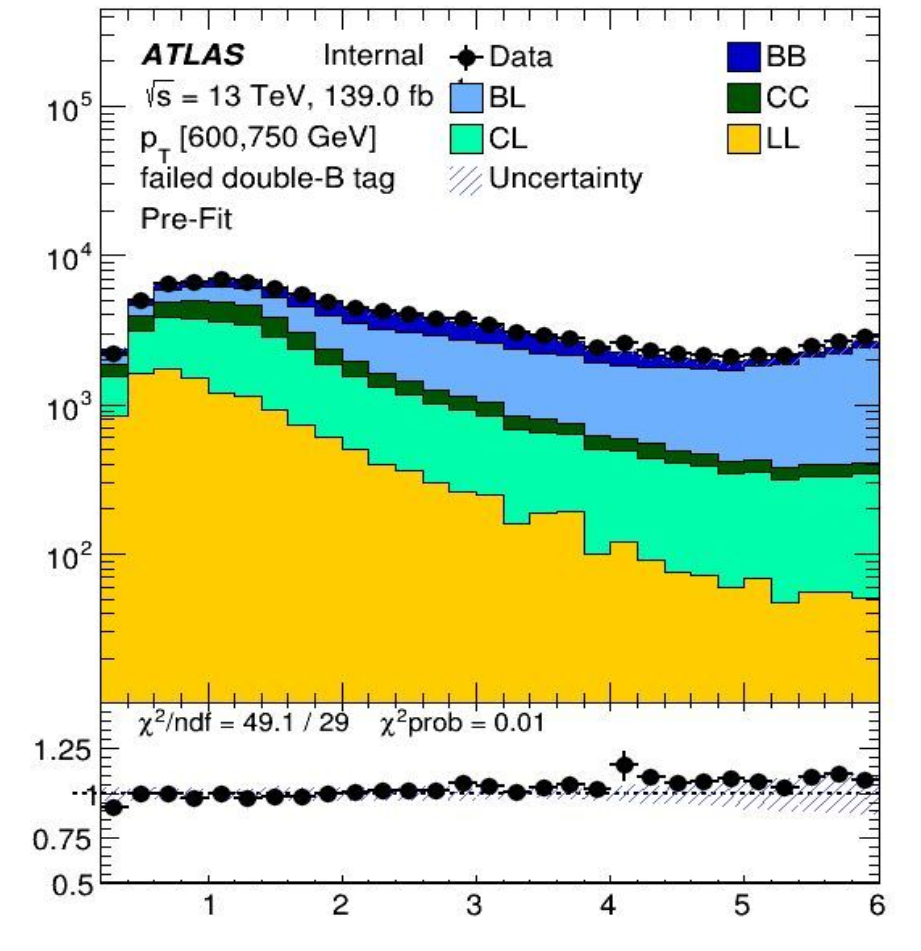
\includegraphics[width=0.485\linewidth]{ftag/sv1Fit/prefit/muon_fail.png} \\
     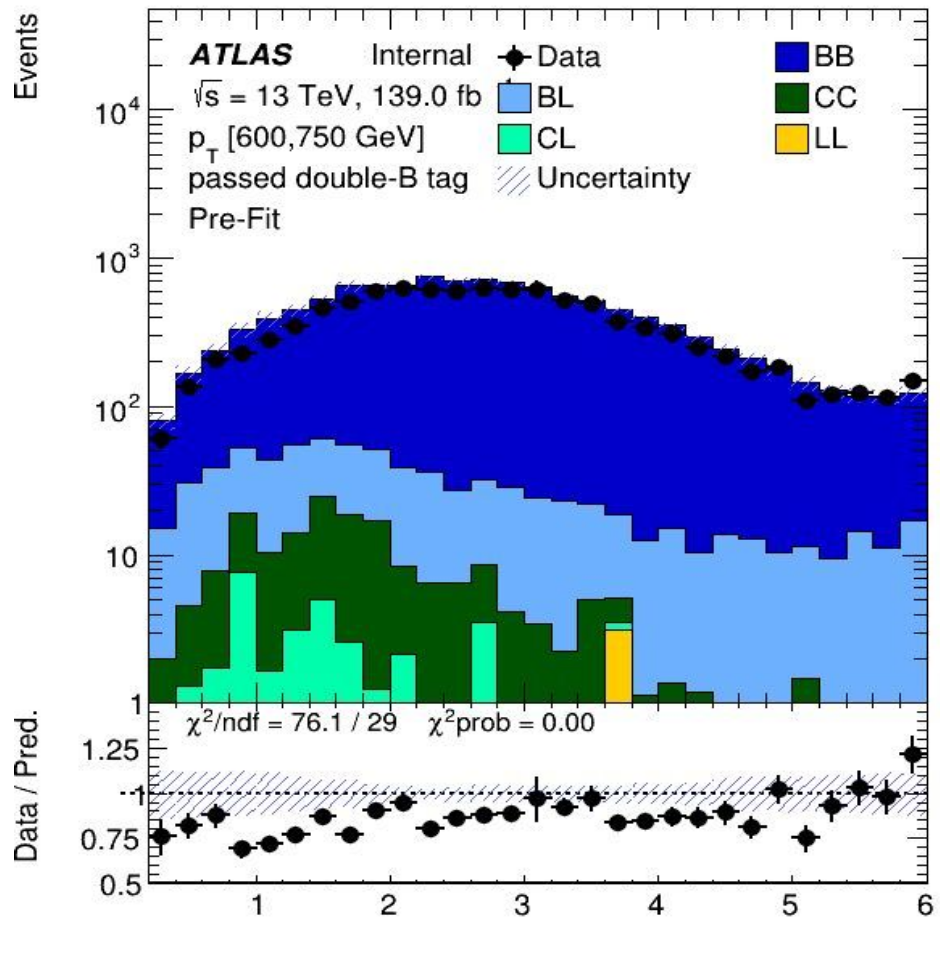
\includegraphics[width=0.485\linewidth]{ftag/sv1Fit/prefit/nonmuon_pass.png}
    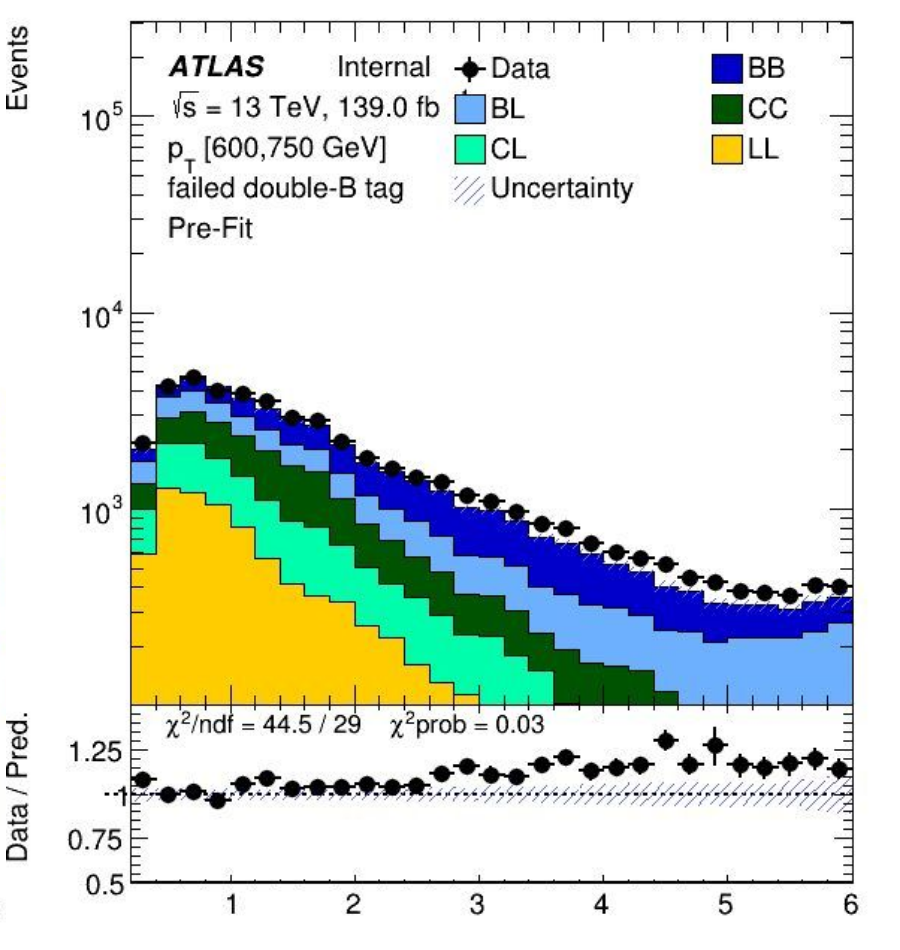
\includegraphics[width=0.485\linewidth]{ftag/sv1Fit/prefit/nonmuon_fail.png} \\
    \caption{The post-fit agreement in the four templates used for the $g\rightarrow b \bar{b}$ calibration with the SV1 mass variable. The top row corresponds to the muon jet and the bottom row to the leading non-muon jet. The left column shows the double-b tagged large-R jet and the right column the anti-tagged jet.}
    \label{fig:postfit_sv1}
\end{figure}

The fit converges and the scale factors obtained in all large-R jet $p_t$ regions is shown in Figure~\ref{fig:sf_sv1}. These are shown to be compatible with those shown in Figure~\ref{fig:sf_sd0}. They are all below unity, and generally compatible within uncertainties.

\begin{figure}
    \centering
    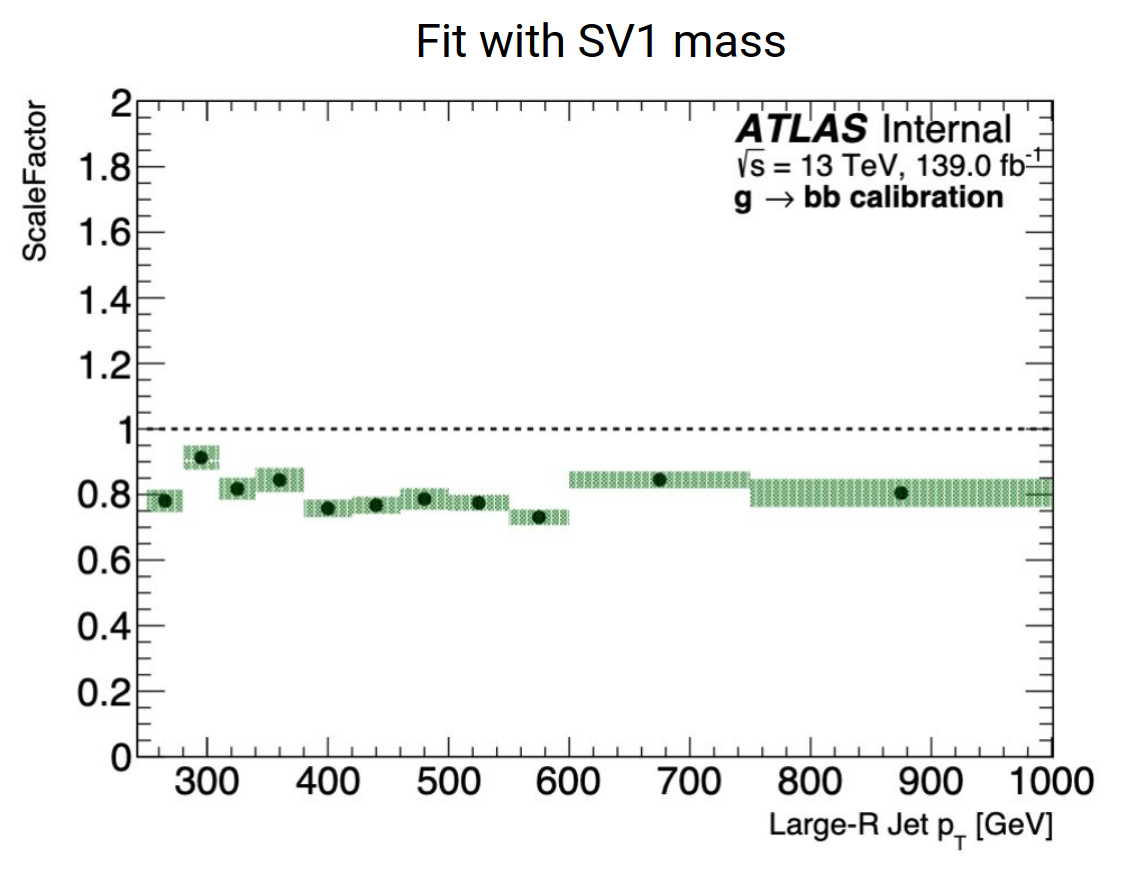
\includegraphics[width=0.5\linewidth]{ftag/sv1Fit/scale_factor.png}
    \caption{The scale factors in each $p_t$ sliced extracted from the $g\rightarrow b\bar{b}$ fit with the SV1 mass.}
    \label{fig:sf_sv1}
\end{figure}

Figures aasdlfòk and alsòkdfjas show the pulls and correlation matrix for the NPs of the fit. These are the same as those found for the mean $s_{d_0}$ fit. 

\begin{figure}
    \centering
    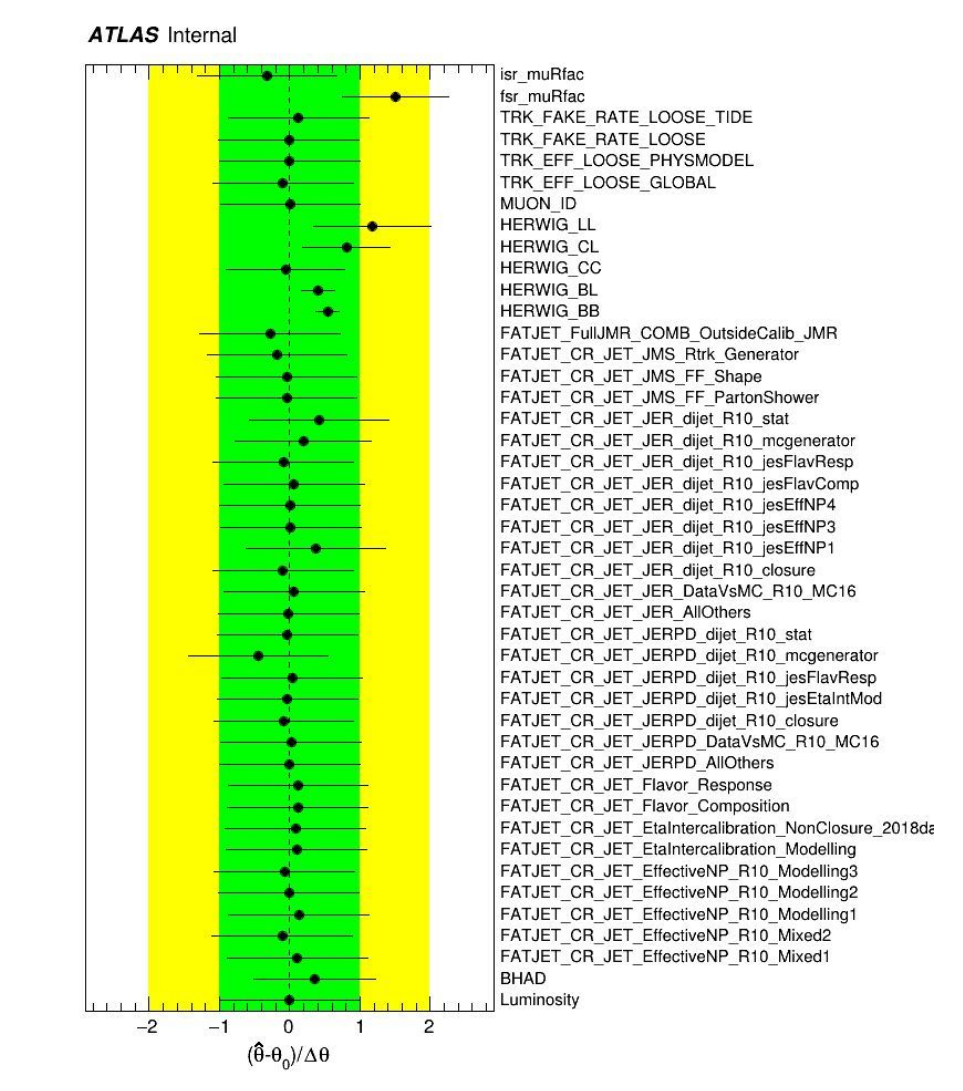
\includegraphics[width=0.8\linewidth]{ftag/sv1Fit/pulls.png}
    \caption{The pulls of the systematic variations affecting the SV1 mass template fit, in the large-R jet $p_t$ region between $600 < p_t/\text{GeV} < 750$.}
    \label{fig:pulls}
\end{figure}

\begin{figure}
    \centering
    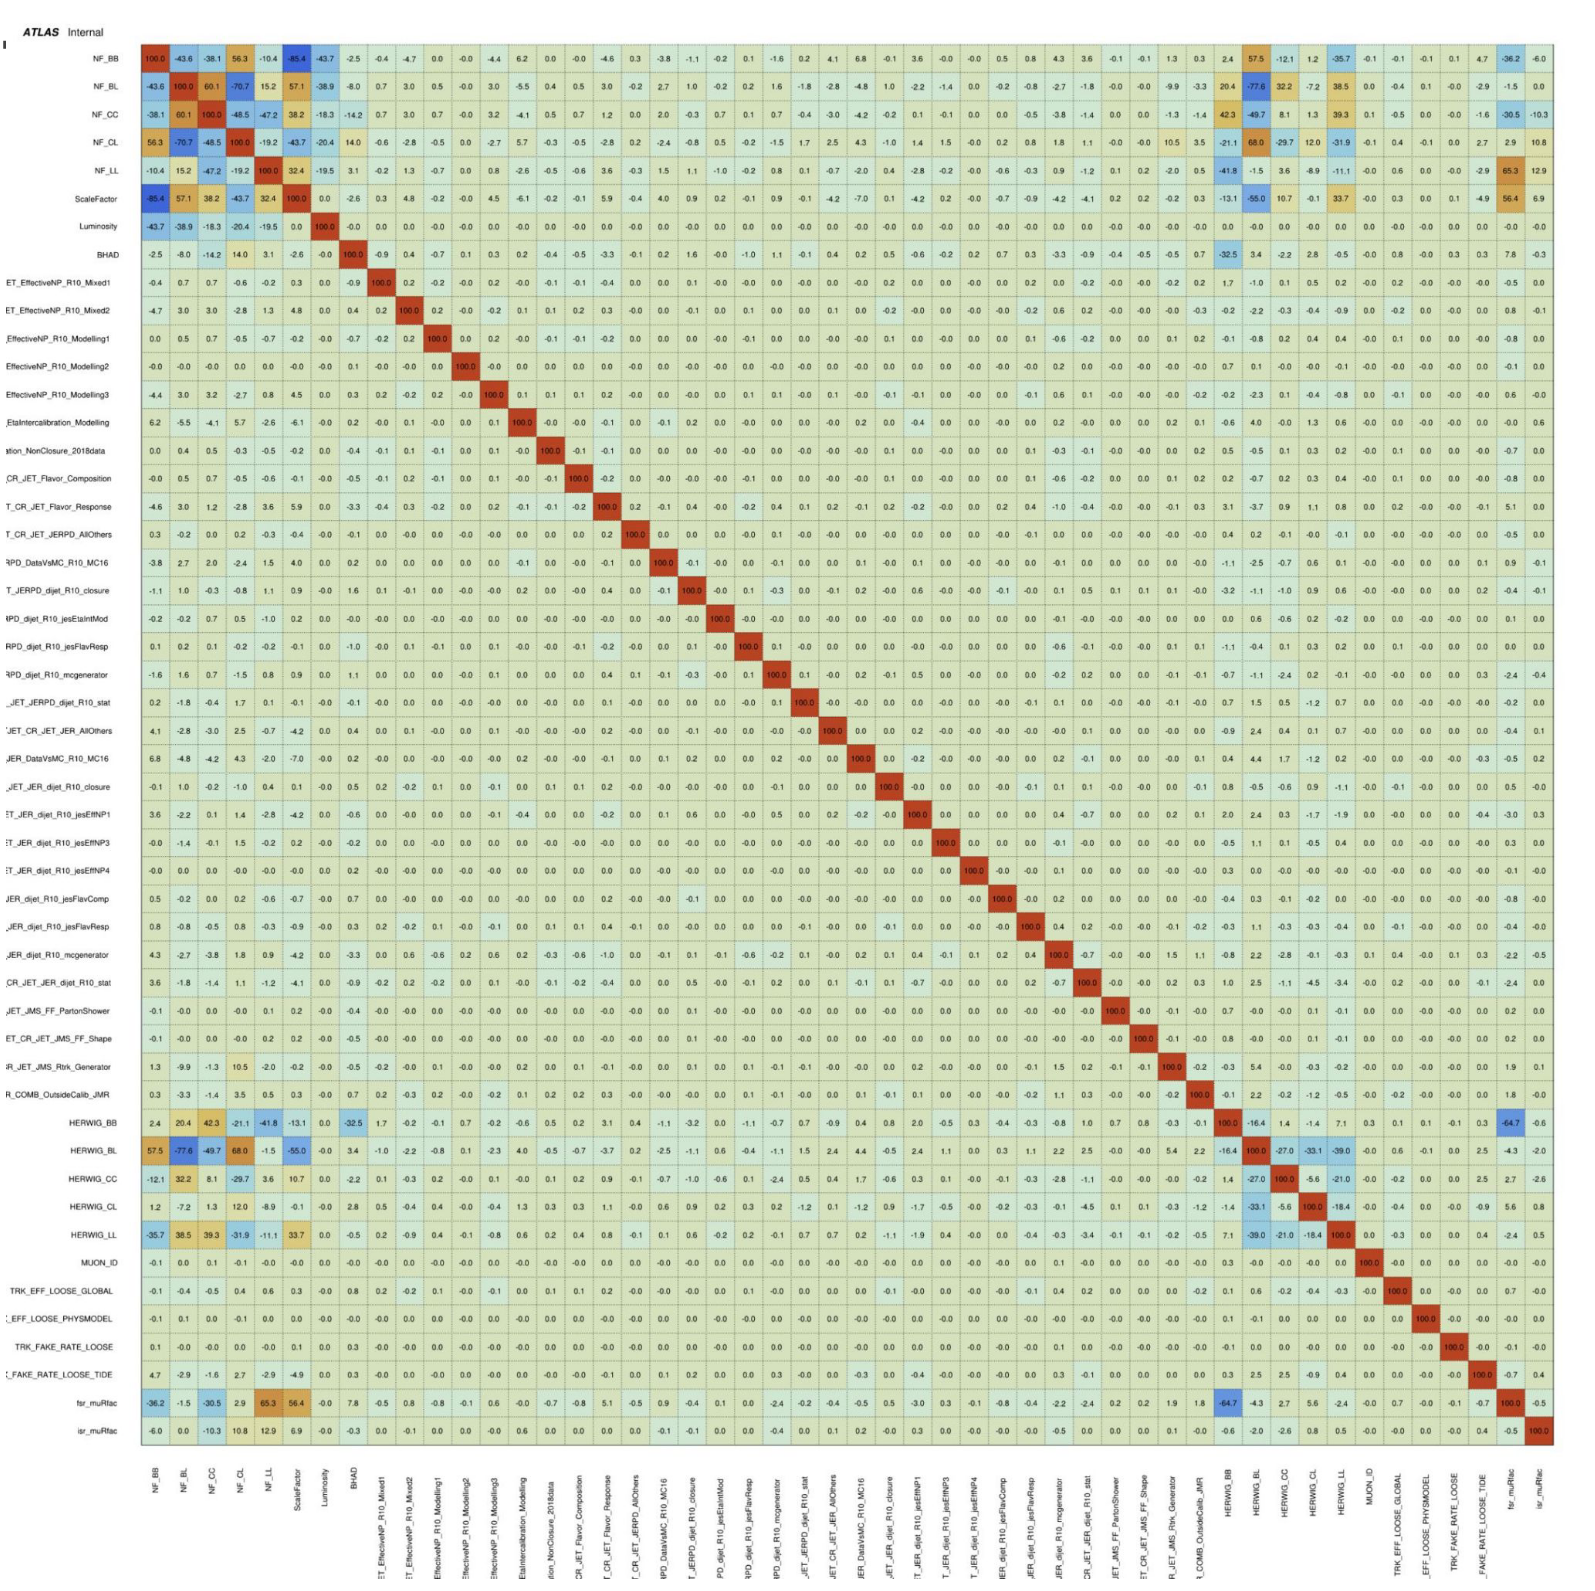
\includegraphics[width=0.8\linewidth]{ftag/sv1Fit/correlation_matrix.png}
    \caption{The correlation matrix of the NPs from the SV1 mass template fit, in the large-R jet $p_t$ region between $600 < p_t/\text{GeV} < 750$.}
    \label{fig:correlation}
\end{figure}


\section{Final comments}

All in all, the Xbb tagger calibration of $g\rightarrow b\bar{b}$ events was successfully completed. The convergence of the fit was proven and results were corroborated with alternate variables.

Some final studies remained on the effect of the smoothing procedure on the fit, and, especially in the SV1 mass fit, the optimisation of the binning and effect of a 3~GeV mass cut on the template fit (to see how the fit behaves in the most populated region of this variable). Many other studies were carried out, such as an optimisation of the flavour template definition, which did not find their way into this thesis.

My work on the calibration was carried out in Software Release 21 in 2022-2023. In 2023, the calibration of the Xbb tagger in this software release was abandoned in favour of the calibration in later releases, based on the GN2 tagger rather than DL1r. 

\chapter{Flavour labelling studies}

Flavour tagging is the identification of heavy flavour jets in data. In particle-level simulations, the identification of heavy flavour jets, or \emph{flavour labelling}, is equally important for a number of reasons. 

First, it is a crucial component of fixed-order calculations involving heavy flavour production. At NNLO and beyond, defining a jet's flavour is highly non-trivial, as effects such as gluon splittings can ``contaminate'' a jet with heavy flavours which do not stem directly from the matrix element. This can be in the form of a soft gluon splitting into a heavy flavour pair within a jet, a wide-angle gluon splitting leading to one of the quarks entering a jet, or a splitting of the form $b\rightarrow gb$, which reduces the $b$-quark (and subsequent hadron) $p_t$ below the threshold for consideration for geometric matching.

\begin{figure}
    \centering
    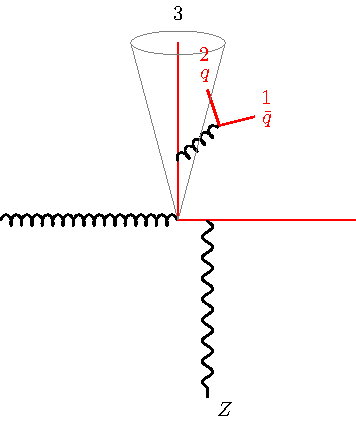
\includegraphics[width=0.5\linewidth]{ftag/NNLO-standard-issue.pdf}
    \caption{A wide-angle gluon splitting to heavy flavours (1,2) in a $Z$+jets event which contaminates the flavour of jet 3~\cite{Caola:2023wpj}.}
    \label{fig:nnlo}
\end{figure}

Were we to assign flavour naively, based solely on the presence of heavy flavour quarks (at parton level) or heavy flavour hadrons within a given jet, such effects would lead to flavour mislabelling. For precision calculations and comparison to data, it is crucial to be able to identify spurious flavour arising from the parton shower.

Accurate flavour labelling is also a critical component of flavour tagging. To train an algorithm, one needs to identify at particle level jets containing heavy flavours, to then, at reconstruction level, be able to identify within the detector simulation those features which allow for the identification of these jets in data. Here, there is some merit in an inclusive definition of flavour, allowing for these contaminations: if one is solely interested in fragmentation studies, it is irrelevant to consider whether the fragmenting heavy flavour quark arises from the matrix element or parton shower. In addition, it is impossible to distinguish these two cases experimentally. However, mislabelling of jets in training can lead to bias since, for example, wide-angle $b\bar{b}$ pairs can lead to the contamination of $c$-jets, considering the fact that $b$-flavour takes priority over $c$. More details will follow in Section \textcolor{red}{Add number}.

In recent years, a number of novel IRC-safe jet clustering algorithms which take flavour into account have been developed to solve this inconsistency. Collectively, these are known as \emph{flavour jet algorithms}. In this Section, we will describe these algorithms and evaluate their impact on several theoretical and experimental aspects of flavour labelling. This section is based off of work initiated at the 2023 Les Houches Workshop~\cite{Huss:2929863} and results published in~\cite{Behring:2025ilo}. 

\section{Current flavour labelling strategies}

Historically, three different strategies for flavour labelling have been used. These are as follows:

\begin{enumerate}
    \item \textbf{Anti-$k_t$ labelling:} A jet is labelled as a heavy flavour jet if a particle containing bottom or charm is found within it, as determined by the jet clustering algorithm (typically anti-$k_t$). This particle may be the quark itself, if the labelling is done at parton level, or else a hadron whose decay has been suppressed.
    \item \textbf{Geometric matching:} This is the strategy used to label jets within ATLAS. It is applied exclusively at hadron level. A jet is labelled as $b$ if a $b$ hadron with $p_t > 5$~GeV is found within a radius of $R < 0.3$ of the jet's axis. The hadron must be one of the initial hadrons formed after hadronisation. The jet is otherwise labelled as a $c$-jet if no $b$ hadron is found, but a $c$ hadron is found satisfying the same requirements.
    \item \textbf{Ghost matching:} This strategy is again applied exclusively at hadron level. The four-momentum of the heavy flavour hadrons found within an event are suppressed to near-zero. The jet clustering algorithm is then applied. If the ghost hadron is found as a constituent of the reclustered jet, the jet is labelled as the flavour corresponding to the hadron species. $B$ flavour takes precedence over $c$ flavour.
\end{enumerate}

As mentioned, however, these flavour labelling strategies are not robust to spurious flavour contributions arising from gluon splittings at NNLO and beyond. To resolve this issue, a number of 
flavour jet clustering algorithms have been proposed.

The first such algorithm, known as \emph{Flavour-$k_t$}, was proposed in 2007 by Banfi, Salam and Zanderighi~\cite{Banfi:2007gu}. This algorithm was never widely adopted as it clusters jets with $k_t$-like kinematics, thus tending to cluster soft particles together.

More recent proposals have succeeded in maintaining jets with anti-$k_t$ like kinematics. In general, these work by identifying flavour pairs which originate from a gluon splitting across the entire event. This is evaluated based on a criterion, which, if satisfied, leads to the cancellation of flavour in the registry of the algorithm. The resulting flavour from these cancellations is what is assigned to the jet, which is clustered according to anti-$k_t$ algorithm. 

The method of combining flavour is known as the \emph{flavour recombination scheme}. Again, there are possible approaches. These include: \emph{any flavour}, \emph{net flavour}, and \emph{mod-2 flavour}. These are described in Table \ref{tab:flavour_recombination_schemes}. 

As flavour is not an IRC safe observable, the any flavour recombination scheme suffers from the problems described above. The flavour assigned based on the net flavour and mod-2 recombination schemes, on the other hand, does not change due to a $g\rightarrow b\bar{b}$ splitting, curing the IRC safety issues.

On the other hand, the any flavour and mod-2 flavour recombination schemes have the benefit of being the most realistic, i.e. they are the ones most which can be most readily implemented in experiment. The mod-2 flavour recombination scheme has the added benefit of being robust against $B-\bar{B}$ oscillations when applied at hadron level.

% Requires: \usepackage{amsmath}
\begin{table}[h]
    \centering
    \begin{tabular}{|l|l|}
    \hline
    \textbf{Scheme} & \textbf{Consider a set of particles flavoured if $\ldots$} \\ \hline
    any flavour & $\sum_i |f_i| > 0$ \\ \hline
    net flavour & $\sum_i f_i \neq 0$ \\ \hline
    mod-2 flavour & $\sum_i |f_i| \equiv 1 \mod 2$ \\ \hline
    \end{tabular}
    \caption{The different flavour recombination schemes used to assign flavour to a jet. Flavoured particles are assigned a value of $f_i = +1$, while flavoured anti-particles are assigned a value of $f_i = -1$. For unflavoured particles, $f_i = 0$. The sum runs over all particles \( i \) under consideration whose flavour should be combined~\cite{Behring:2025ilo}. }
    \label{tab:flavour_recombination_schemes}
\end{table}

\section{The Next Generation of Algorithms}

We are now ready to describe the flavour jet algorithms in more detail. There are four such algorithms. They can all make use of either the net flavour or mod-2 flavour recombination schemes to maintain IRC safety. Throughout this chapter, the net flavour recombination scheme has been used unless otherwise stated. When results at hadron level are shown, it is understood that the flavour jet algorithms require undecayed heavy hadrons in order to meaningfully ascribe flavour to jets.

\subsection{Soft-drop flavour (SDF)}

This algorithm uses which uses a soft-drop criterion to determine whether a flavour pair originates from a gluon splitting~\cite{Caletti:2022hnc}. Starting from a jet clustered with any algorithm, the jet is reclustered using the \code{JADE} algorithm. At each step during the clustering procedure, the soft-drop flavour algorithm requires that the particles $i$ and $j$ pass the soft-drop criterion (\textcolor{red}{add ref.}) with $\beta > 0$ and $z_\text{cut} < \frac{1}2$. The values of $z_\text{cut} = 0.1$ and $\beta = 1$ or $\beta = 2$ are typically chosen. If the grooming requirement is satisfied, the flavour within the jet is summed according to some recombination scheme, and the JADE clustering proceeds to the next step. If it fails, the softer branch is groomed before proceeding to the next step.  

%io uso sempre beta = 1, devo controllare negli studi teorici

The JADE reclustering step necessarily entails a modification of anti-$k_t$ kinematics, assuming the initial jet considered was clustered with that algorithm. The modification is modest and often negligible in practice. 

\subsection{Flavoured anti-$k_t$ (CMP)}

The CMP algorithm~\cite{Czakon:2022wam} modifies the distance measure used in anti-$k_t$ (\textcolor{red}{add reference}) in order to capture soft, flavoured particles. Specifically, the distance measure $d_{ij}$ is modified through a damping function $S_{ij}$

\begin{equation}
    d_{ij}^{(\text{flavoured})} = d_{ij}^{(\text{standard})} \times 
    \begin{cases} 
      S_{ij}, & \text{if both } i \text{ and } j \text{ have nonzero flavour of opposite sign and magnitude,} \\
      1, & \text{otherwise.}
    \end{cases}
    \label{eq:flavoured_distance}
\end{equation}
which is applied exclusively to flavoured particles. The damping function is required to vanish for soft quark pairs, compared to the scale of the hard process. The function chosen which satisfies these properties is

% Requires: \usepackage{amsmath}
\begin{equation}
\begin{aligned}
    S_{ij} &= 1 - \theta \left(1 - \kappa_{ij}\right) \cos\left(\frac{\pi}{2} \kappa_{ij}\right) \\
    \text{with} \quad \kappa_{ij} &\equiv \frac{1}{a} \sqrt{\frac{\Omega_{ij}^2}{\Delta R^2}} \frac{p^2_{t,i} + p^2_{t,j}}{2p^2_{t,\max}} \\
    \text{and} \quad \Omega_{ij}^2 &= 2 \left[ \frac{1}{\omega^2} \left( \cosh(\omega \Delta y_{ij}) - 1 \right) - \left( \cos \Delta \phi_{ij} - 1 \right) \right].
\end{aligned}
\label{eq:cmp}
\end{equation}

Here, $\theta$ is the Heaviside function, $p_{t, \text{max}}$ is some hard scale, $a$ is a parameter used for tuning, and $\omega$ is a parameter which regulates the distance measure in such a way as to ensure IRC safety. The values of $a = 0.1$, $\omega = 2$ are adopted throughout and $p_{t,\text{max}}$ is dynamically set to the $p_t$ of the hardest subjet at each step in the clustering procedure.

With such a damping function, the CMP algorithm reduces to the anti-$k_t$ algorithm in the absence of soft flavour pairs, and modifies the kinematics slightly when they are present. We can thus speak of \emph{approximate} anti-$k_t$ kinematics, though the modifications are often negligible.

\subsection{Flavour dressing (GHS)}

As the name implies, the flavour dressing (GHS) algorithm~\cite{Gauld:2022lem} aims to decorate a set of jets with flavour. The algorithm starts with a set of flavour-agnostic jets clustered with an algorithm of choice and all particles which make up a given event. If the particle $p_i$ is a constituent of jet $j_k$, the distance $d(p_i, j_k)$ is saved. The distance between particles $p_i$ and $p_j$ $d(p_i, p_j)$ is saved as well if both particles are flavoured or if one is flavoured and they are both associated to the same jet. 

If $d(p_i, p_j) < d(p_i, j_k)$, the particle $k_{ij} = p_i + p_j$ is formed by summing the four-momenta and flavour content of the two particles. In the record of saved distances, $p_i$ and $p_j$ are replaced by $k_{ij}$.

If instead $d(p_i, p_j) > d(p_i, j_k)$, the particle $p_i$ is assigned to jet $j_k$ and all other records contains $p_i$ are discarded.

Finally, if the beam distance $d(p_i, B)$ is smaller than both $d(p_i, p_j)$ and $d(p_i, j_k)$, all saved distances containing $p_i$ are discarded.

The distances considered are:
\begin{gather}
    \label{uik}
    d(p_i, p_k) = \max(p_{ti}, p_{tk})^{\alpha} \min(p_{ti}, p_{tk})^{2-\alpha} \Omega_{ik}^2 \\
    d(p_i, B_{\pm}) = \max \left( p_{t_i}^{\alpha}, p_{t_{B_{\pm}}}^{\alpha}(y_i) \right) \min \left( p_{t_i}^{2-\alpha}, p_{t_{B_{\pm}}}^{2-\alpha}(y_i) \right)
\end{gather}
where $B_\pm$ takes into account the direction of positive/negative rapidity and
\begin{equation}
    p_{tB_\pm} = \max\left(p_{ti}^\alpha, p_{tB_\pm}^\alpha(y_i)\right)\min\left(p_{ti}^{2-\alpha}, p_{tB_\pm}^{2-\alpha}(y_i)\right),
\end{equation}
with $\alpha$ a parameter set to 1, $\Theta(0) = 1/2$,  and $\Delta y_{j_k} = y_{j_k} - y$. $\Omega^2_{ik}$ takes the same form as in Eq.~\ref{eq:cmp}. The parameter $\omega$ is set to 2 as default. To ensure IRC safety, the parameters must be chosen such that $\omega > 2 - \alpha$.

This procedure is iterated until the set of saved distances is empty. The flavour of a jet is then the sum of that of the particles belonging to it. The flavoured jets obtained in this way maintain the initial kinematics of the flavour-agnostic algorithm, such as anti-$k_t$. This algorithm has the added benefit of potentially being applicable experimentally, as the flavoured particles can be proxies such as reconstructed secondary vertices.

\subsection{Interleaved flavour neutralisation (IFN)}

The IFN algorithm~\cite{Caola:2023wpj} searches for flavour to cancel throughout the entire event at each step of the clustering procedure. While clustering a jet with a given algorithm, when combining the particles $i$ and $j$ with $p_{ti} < p_{tj}$ and with $i$ flavoured, the IFN algorithm searches for other flavoured particles through a list $L$ of flavoured subjets $k \in L$. If the distance between $i$ and $k$ satisfies Eq.~\ref{uik}, the flavour of $i$ and $k$ is neutralised and is treated as null. This is illustrated in Figure~\ref{fig:ifn}.

The result is a set of jets with the exact kinematics of the algorithm used to cluster them, usually anti-$k_t$. The algorithm depends on same two parameters as the GHS algorithm, $(\alpha, \omega)$, and the same choice of $(1,2)$ is possible, though the default choice is $(2,1)$.

\begin{figure}
    \centering

    \subfloat[\label{a}]{%
        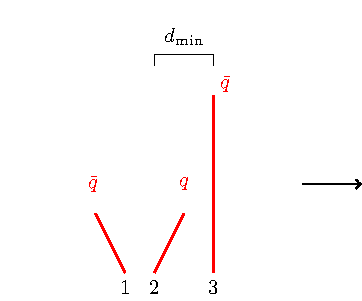
\includegraphics[width=0.245\linewidth]{ftag/neutralisation-a.pdf}    
    }
    \subfloat[\label{b}]{%
        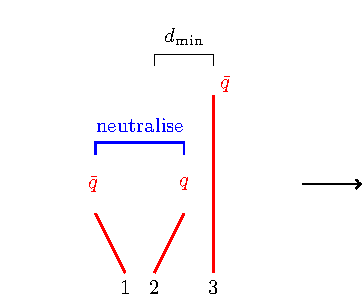
\includegraphics[width=0.245\linewidth]{ftag/neutralisation-b.pdf}    
    }
    \subfloat[\label{c}]{%
        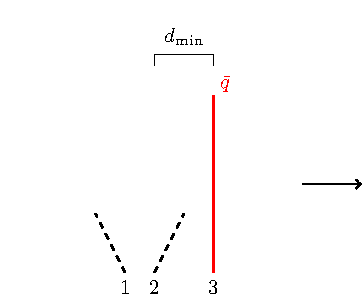
\includegraphics[width=0.245\linewidth]{ftag/neutralisation-c.pdf}    
    }
    \subfloat[\label{d}]{%
        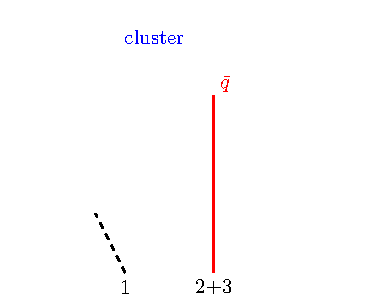
\includegraphics[width=0.245\linewidth]{ftag/neutralisation-d.pdf}    
    }
    \caption{The steps in flavour neutralisation in the IFN algorithm. In Figure~\ref{a}, particles 1 and 2 are a heavy flavour pair arising from a soft gluon splitting, and particles 2 and 3 are meant to be clustered. In Figure~\ref{b}, it is found that the particles 1 and 2 satisfy the distance ~\ref{uik}, and so their flavour is neutralised as shown in Figure~\ref{c}. The clustering can thus proceed as in Figure~\ref{d}, combining particles 2 and 3 with no flavour~\cite{Caola:2023wpj}.}
    \label{fig:ifn}
\end{figure}

\section{Flavoured jet algorithms: A comparative study}

At the 2023 Les Houches Workshop, a detailed study of the differences between the flavour jet algorithms was initiated, from various points of views. This section is dedicated to selected findings from those studies, published in~\cite{Behring:2025ilo}.

\subsection{Flavour recombination scheme}
\label{flav recomb}
To understand the effect of modifying the choice of flavour recombination scheme from any flavour to the more recent proposals which do not break IRC safety, a study on hadron-level simulated data was carried out. Here, $pp \rightarrow Z+\mu^+\mu^-$+jet matrix elements were calculated at NLO and showered using Herwig7~\cite{Bellm:2015jjp} and Sherpa~\cite{Sherpa:2024mfk} at $\sqrt{s} = 13$~TeV. Two different Herwig7 showers were carried out, one using the Lund string hadronisation model, and the other using the cluster hadronisation model. Jets were clustered suppressing the decays of the heavy hadrons and with a radius of 0.5. They are required to have $p_t > 30$~GeV and rapidity $\vert y \vert < 2.4$. The transverse momentum of the individual muons and the dimuon pair must be greater than 20~GeV $p_t^\mu > 20$~GeV and $p_t^{\mu\mu} > 20$~GeV. The mass of the dimuon pair must be close to that of the $Z$ $77 < m^{\mu\mu}/\text{GeV} < 111$. Individual muons are also required to be in the central region $\vert y^\mu \vert < 2.4$. $b$-jets and $c$-jets were identified using ghost and cone labelling with the any flavour recombination scheme, and with anti-$k_t$ labelling using the mod-2 flavour recombination scheme.

Figure~\ref{fig:summary_ppzj_nlops_bottom_exp} shows the leading $b/c$-jet distributions for these predictions with anti-$k_t$, ghost, and cone labelling. For both the Sherpa and Herwig7 showers, the mod-2 flavour recombination scheme leads to a reduction in the number of jets labelled as $b/c$ due to the elimination of heavy flavour pairs stemming from soft gluon splittings. This reduction increases as jet $p_t$, since the number of soft gluon splitting increases as the energy scale increases. The effect is also more pronounced for $c$-jets, as the number of $g\rightarrow c\bar{c}$ splittings is expected to be greater than $g\rightarrow b\bar{b}$ due to the masses of the particles, and for jets labelled with ghost labelling. In this case, the difference compared to cone labelling is attributed to the labelling itself: in cone labelling, a radius of $\Delta R < 0.3$ between the hadron and jet is considered, whereas for ghost labelling the radius is effectively equal to that of the jet radius.

\begin{figure}
    \centering
    \includegraphics[width=0.5\linewidth,page=3]{ftag/summary/ppzj_bottom_nlops_comparisons_exp.pdf}%
    \includegraphics[width=0.5\linewidth,page=3]{ftag/summary/ppzj_charm_nlops_comparisons_exp.pdf}
    \caption{NLO+PS predictions from Sherpa and Herwig7 for $pp \to \Z + b$ (left) and $pp \to \Z + c$ (right) in central kinematics. Different experimentally inspired jet labelling algorithms are compared to the anti-$k_t$ algorithms with mod-2 recombination for the transverse momentum of the leading $b$/$c$ jet. Additionally, differences between the cluster and string hadronisation model for Herwig7, as well as parton and hadron level for Sherpa, are shown~\cite{Behring:2025ilo}.}
    \label{fig:summary_ppzj_nlops_bottom_exp}
\end{figure}

The labelling is effectively identical for both hadronisation models considered for the Herwig7 showers. When comparing parton/hadron level, some differences arise between jets labelled with ghost/cone and anti-$k_t$. These differences are more marked for $c$-jets.

\subsection{Neutralisation of flavour from gluon splittings}

We turn our attention now to the differences between the various flavour jet algorithms. Although they were all designed to address the same concern, the exact approach varies. 

Figure~\ref{fig:summary_ppzj_lops_bottom} shows LO+PS $Z+$jet events produced with selections similar to those in Section~\ref{flav recomb} using Pythia v8.306~\cite{Pythia:2022pfr} without hadronisation. It compares the number of $b$-jets found using the flavour jet algorithms with certain configuartions of parameters to those found with anti-$k_t$ labelling. It is clear that the number of jets identified is lowest for the IFN algorithm with $\alpha = 2$.

\begin{figure}
    \centering
    \includegraphics[width=0.49\linewidth,page=2]{ftag/lops_ppzjet/pythia-Zj-flav-algs.pdf}    \caption{The ratio, to net-flavour anti-$k_t$ (in red), of IFN ($\alpha=1$ and $\alpha=2$, blue), CMP ($a=0.1$, green), GHS ($\alpha=1$, $\omega=2$, black) and SDF ($\beta=2$, $z_{\cut}=0.1$, yellow), for the transverse momentum of the leading $b$-labelled jet $p_{t,b\text{-jet}}$~\cite{Behring:2025ilo}.}
    \label{fig:summary_ppzj_lops_bottom}
\end{figure}

This effect is attributed to the neutralisation of the most heavy flavour pairs coming from soft gluon splittings. To prove this, Figure~\ref{fig:lops_ppzjet_scatter_all}
 shows a series of scatter plots of a subset of the generated $Z$+jet events with at least two $b$-quarks at parton level and leading $b$-jet $p_t > 200$~GeV, as decided by anti-$k_t$ labelling. On the x-axis, the angular distance between the $b$-quarks is shown, while on the y-axis the $p_t$ fraction of the jet carried by the leading $b$-quark in the jet $p_{t,b}/p_{t, b\text{-jet}}$ is reported. Events where the flavour content originates from wide-angle, soft gluon splittings populate mostly the bottom-left corner. The exact truth origin of all events in the plot is shown in Figure~\ref{fig:z+j_lops_truth}, showing true $Z+b$ events, $Z+q$ events containing mostly light quarks where $b$-jets tend to originate from gluon splittings, and $Z+g$ events, where $b$-jets arise from both soft and hard gluon splittings. The other figures show the events labelled as $b$-jets by anti-$k_t$ and each individual flavour jet algorithm in grey, or just by anti-$k_t$ in red. It is clear that IFN, as declared, is better at identifying genuine $b$-jets than the other algorithms.

\begin{figure}
    \centering
    \subfloat[Truth\label{fig:z+j_lops_truth}]{%
        \includegraphics[width=0.48\linewidth, page=5]{ftag/lops_ppzjet/pythia-Zj-scatter.pdf}    
    }\\
    \subfloat[IFN\label{lops_figb}]{%
        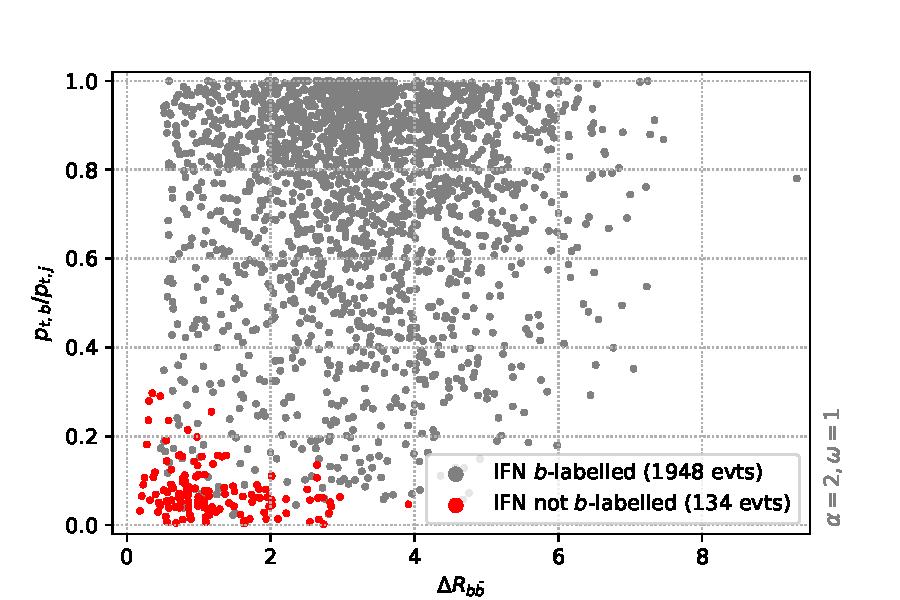
\includegraphics[width=0.48\linewidth, page=1]{ftag/lops_ppzjet/pythia-Zj-scatter.pdf}    
    }  
       \subfloat[CMP\label{lops_figc}]{%
        \includegraphics[width=0.48\linewidth, page=2]{ftag/lops_ppzjet/pythia-Zj-scatter.pdf}    
    }\\    \subfloat[GHS\label{lops_figd}]{%
        \includegraphics[width=0.48\linewidth, page=3]{ftag/lops_ppzjet/pythia-Zj-scatter.pdf}    
    }    \subfloat[SDFlav\label{lops_fige}]{%
        \includegraphics[width=0.48\linewidth, page=4]{ftag/lops_ppzjet/pythia-Zj-scatter.pdf}    
    } 
    
    \caption{$Z+$jets events with at least 2 $b$-quarks and a $b$-jet with $p_t > 200$~GeV as identified with anti-$k_t$ as a function of $\Delta R_{b\bar{b}}$ and
      $p_{t,b} / p_{t,b\text{-jet}}$. In Figure~\ref{fig:z+j_lops_truth} the truth origin of these events is shown. In Figures~\ref{lops_figb}$-$\ref{lops_fige}, the label assigned by the selected jet algorithm vs. anti-$k_t$ is shown, with grey events labelled as $b$ by
      both net flavour anti-$k_t$ and the algorithm under consideration and red events labelled as $b$ by net flavour anti-$k_t$, but not by the flavoured algorithm~\cite{Behring:2025ilo}.}
    \label{fig:lops_ppzjet_scatter_all}
\end{figure}

The results shown in Figure~\ref{fig:summary_ppzj_lops_bottom} are valid also at NLO, as shown in the top panels of Figure~\ref{summary_ppzj_nlops_bottom} for $b/c$-jets. In this case, the Sherpa and Herwig7 were used as parton showers along with the mod-2 flavour recombination scheme. The figure also shows how the results remain valid at hadron level independently of the hadronisation model chosen. When comparing the results for the Sherpa sample at hadron and parton level, differences in the trends observed for the flavour jet algorithms arise for high-$p_t$ $c$-jets. These are attributed to ... \textcolor{red}{Do we know? Not commented in appendix C of paper.}

\begin{figure}
    \centering
    \includegraphics[width=0.5\linewidth,page=3]{ftag/summary/ppzj_bottom_nlops_comparisons.pdf}%
    \includegraphics[width=0.5\linewidth,page=3]{ftag/summary/ppzj_charm_nlops_comparisons.pdf}
    \caption{NLO+PS predictions from Sherpa and Herwig7 for $pp \to \Z + b$ (left) and $pp \to \Z + c$ (right) in central kinematics. Different jet algorithms (CMP$\Omega$ -- green, SDF -- light blue, GHS -- yellow, IFN -- red) are compared for the transverse momentum of the leading $b$/$c$ jet. Additionally, differences between the cluster and string hadronisation model for Herwig7, as well as parton and hadron level for Sherpa, are shown. The vertical bars indicate statistical uncertainties~\cite{Behring:2025ilo}.}
    \label{fig:summary_ppzj_nlops_bottom}
\end{figure}

\subsection{Effect of constituents}
\label{eo constituents}
We consider now the effect of the constituents used in the jet definition on flavour labelling. In experimental collaborations, such as ATLAS and CMS, flavour labelling is done on jets whose fiducial definitions match the experimental reality as closely as possible using cone or ghost labelling. This means that the final states considered when clustering jets consist of all stable, visible particles in the event, and flavour is assigned to these jets. This is in contrast to the jet definitions used by theorists where in many instances the jets are not clustered in the most realistic manner, i.e. when suppressing hadron decay for anti-$k_t$ labelling. 

This difference has critical implications for jet kinematics. Consider $Z+b\bar{b}$ and $Z+c\bar{c}$ events generated at LO with MadGraph\_aMC\@NLO v3.5.8~\cite{Alwall:2014hca} and showered with Pythia v8.313. Hadronisation was allowed to occur. Jets are clustered following the prescription used by the ATLAS AntiKt04TruthJet collections, namely with all stable, visible particles within $\vert \eta \vert < 2.5$ and with radius $R = 0.4$. An exception is made for jets clustered with the flavour jet algorithms. In this case, heavy hadron decays are artificially suppressed as required by the algorithms. The undecayed hadrons are treated as stable.

Jets are required to fall within the central region, i.e $\vert y \vert $ < 2.5 and have $p_t > 20$~GeV. $Z\rightarrow l^+l^-$ events are considered, where the individual leptons are required to have $p_t^{lep} > 27$~GeV, $\vert \eta_{lep} \vert < 2.5$ and dilepton mass $76 < m_{ll}/\text{GeV} < 106$. Events with at least one $b/c$-jets are selected. The two leading $b/c$-jets are selected when multiple labelled jets are found.   

As can be seen in Figure~\ref{fig:decay}, there are significant kinematic differences between the labelled jets as $b/c$ with ghost and cone labelling and with the flavour jet algorithms. These differences are accentuated at low-$p_t$.

\begin{figure}
    \centering
    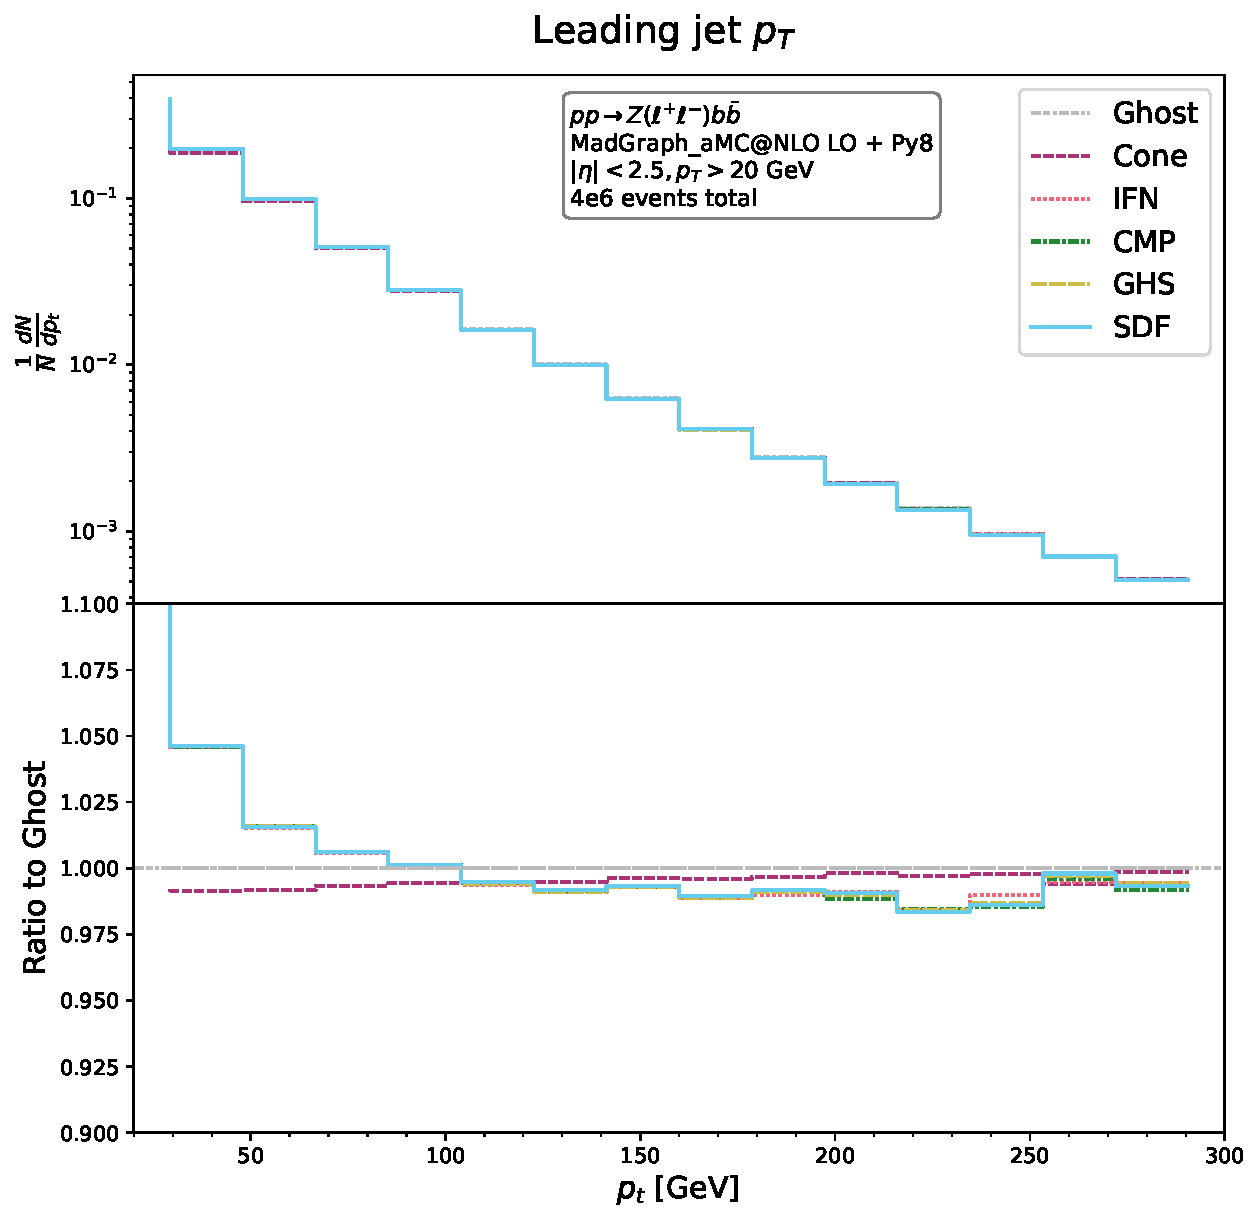
\includegraphics[width=0.485\linewidth]{ftag/leadJetPt_decayed_b.pdf}
    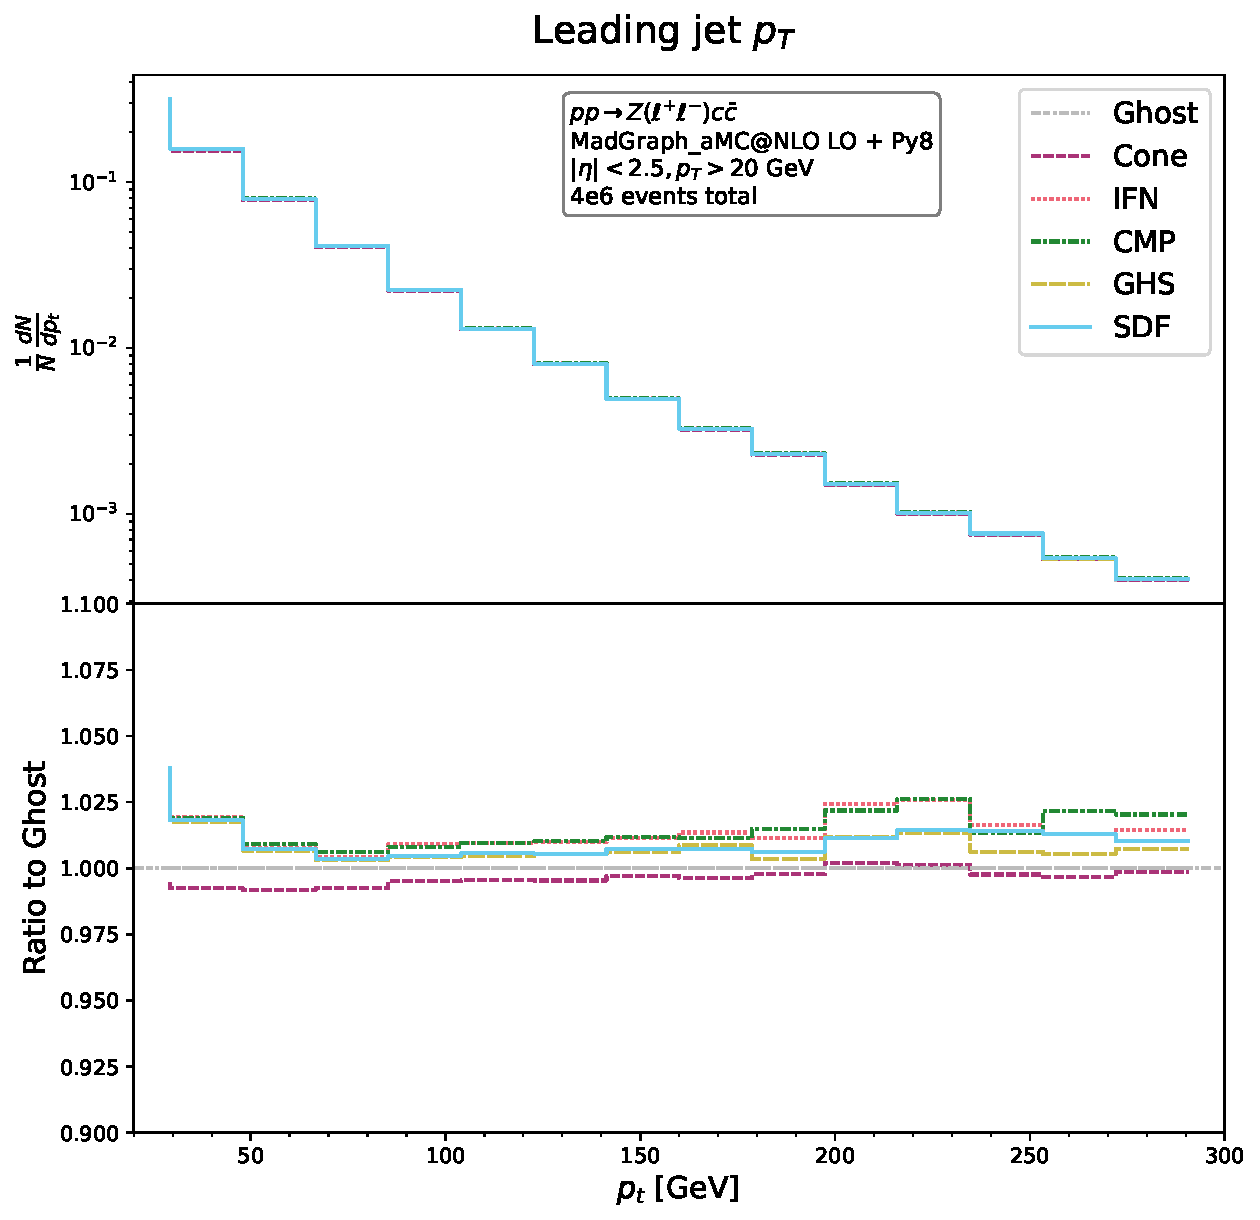
\includegraphics[width=0.485\linewidth]{ftag/leadJetPt_decayed_c.pdf}
    \caption{The $p_t$ distribution of leading 
    $b$-jets (left) and leading $c$-jet (right) identified with
the experimental ghost and cone labelling schemes with stable final state particles and flavoured jet algorithm with undecayed heavy hadrons. Ratios are compared to the distribution for jets obtained with ghost labelling~\cite{Behring:2025ilo}.}
    \label{fig:decay}
\end{figure}

This is attributed to the difference in constituents. Figure~\ref{fig:undecay} shows how, if the constituent definition prescribed by the flavour jet algorithms is used in all labelling schemes, the kinematic differences disappear and the expected behaviour is observed throughout the entire $p_t$ spectrum.

\begin{figure}
    \centering
    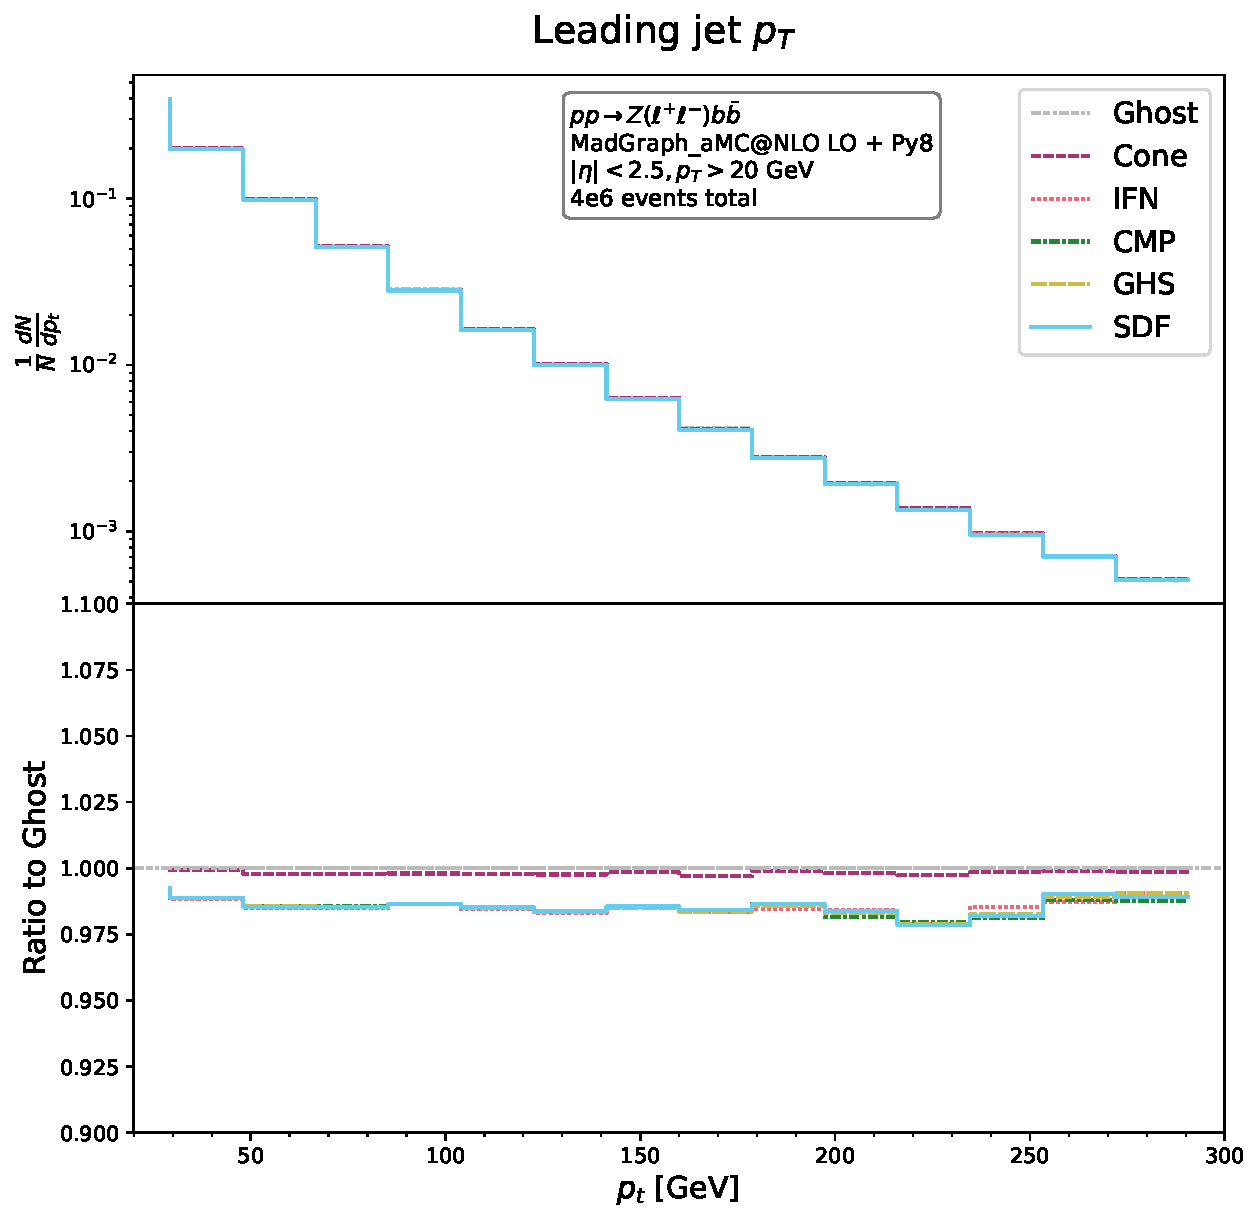
\includegraphics[width=0.485\linewidth]{ftag/leadJetPt_undecayed_b.pdf}
    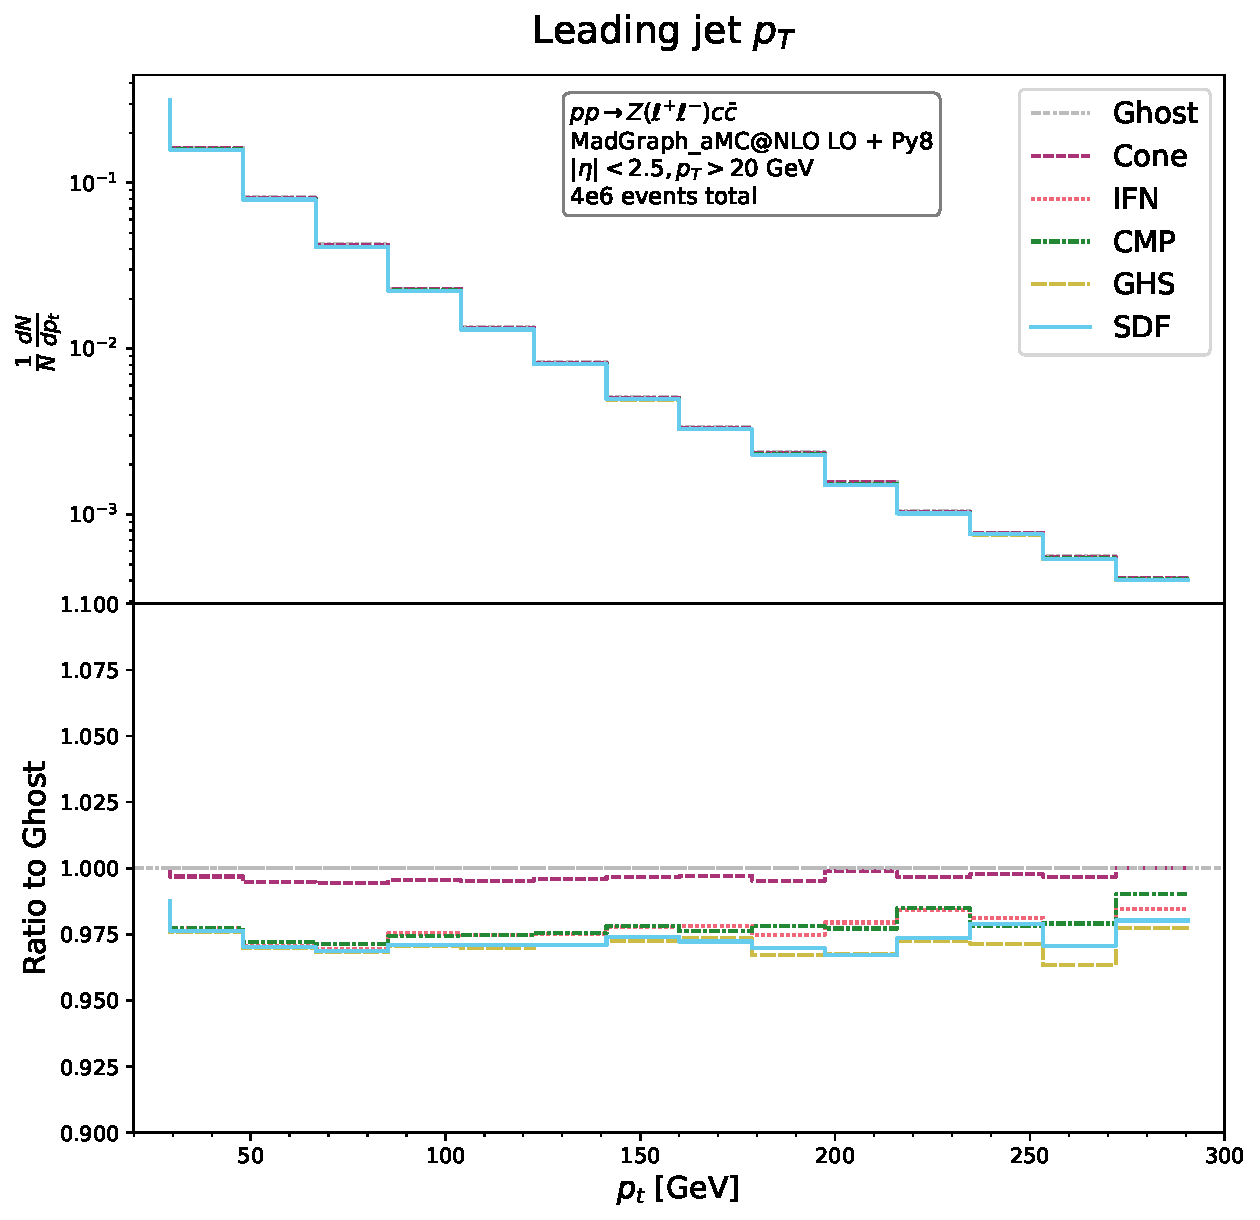
\includegraphics[width=0.485\linewidth]{ftag/leadJetPt_undecayed_c.pdf}
    \caption{The $p_t$ distribution of leading 
    $b$-jets (left) and leading $c$-jet (right) identified with
the ghost cone labelling schemes and the flavoured jet algorithms, all with undecayed heavy hadrons. Ratios are compared to the distribution for jets obtained with ghost labelling~\cite{Behring:2025ilo}.}
    \label{fig:undecay}
\end{figure}

These results highlight the importance of harmonisation. Ideally, the new flavour algorithms would be adopted by experimental collaborations, at least in the context of precision physics in order to more accurately predict relevant cross sections for the production of heavy flavour particles, correcting for effects such as gluon splittings. If this is to be done, the collaborations must either revisit their truth-level jet definitions in order to take into account kinematic effects arising from the difference in constituents, or implement an additional unfolding-like step to correct for the differences that arise when using these novel labelling schemes. 

\subsection{Consequences for Flavour Tagging algorithm training}
Other practical implications of the inadequacy of the current flavour labelling strategies in use in experiments can be found in flavour tagging training. 

Let us consider one of the samples used for training by the ATLAS Collaboration, $Z^\prime \rightarrow c\bar{c}$. The events are generated at LO and showered with Pythia, and jets are required to have $\vert \eta \vert < 2.5$ and $p_t > 250$~GeV. In all cases, heavy hadron decays are suppressed. 

In Figure~\ref{{fig:ATLAS-FTAG-comparison}}, we show how for intermediate values of $p_t$ in this range, between 1.5-4~TeV, there is a surplus of jets labelled as $c$-jets by the flavour jet algorithms and anti-$k_t$ labelling scheme compared to cone. If instead we consider $b$-jet labelling, the expected behaviour is found, namely a surplus of jets labelled by the cone algorithm throughout the entire $p_t$ spectrum. Figure~\ref{b_or_c} shows the reason behind this anomaly: soft  $g \rightarrow b\bar{b}$ contaminate the $c$-jets with $b$ flavour. Algorithms which more aggressively remove gluon splittings will tend to assign the correct flavour, while those which less aggressively remove these splittings will tend to assign a dual ``$bc$'' flavour. As $b$ flavour is assigned preferentially over $c$ flavour, this leads to a mislabelling. When considering the dual flavour, the expected behaviour returns.

\begin{figure}
    \centering
    \subfloat[\label{or_b}]{
    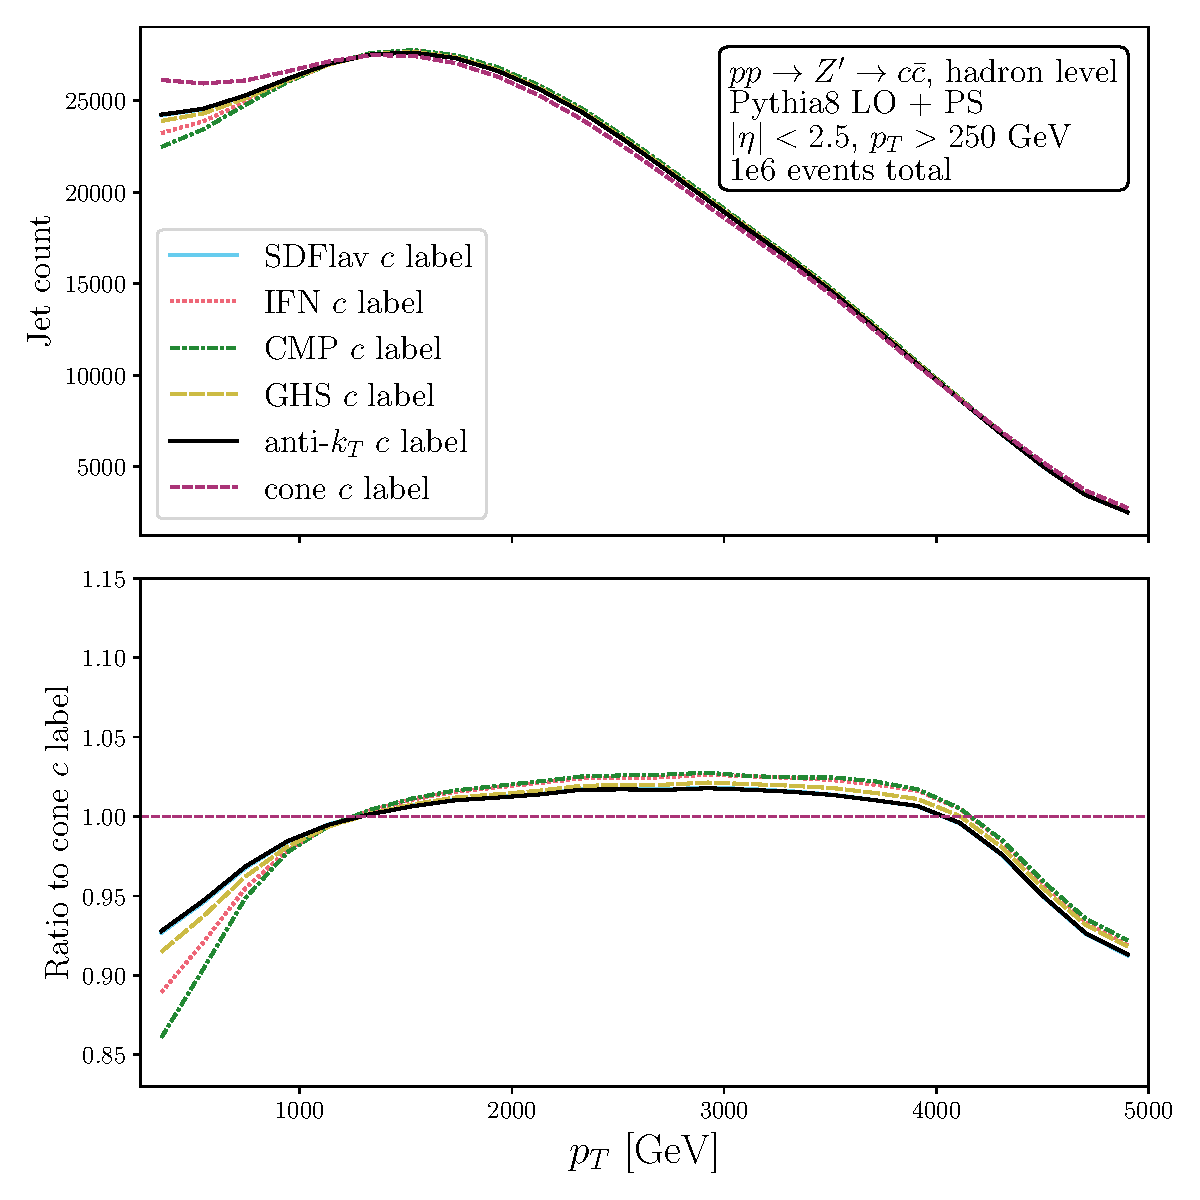
\includegraphics[width=0.49\linewidth]{ftag/NETno-grey-lineBLACKANTIKT-MAINCIFN-CMP-ATLAS-compare-pt-with-ratio.pdf} }
    \subfloat][\label{or_c}]{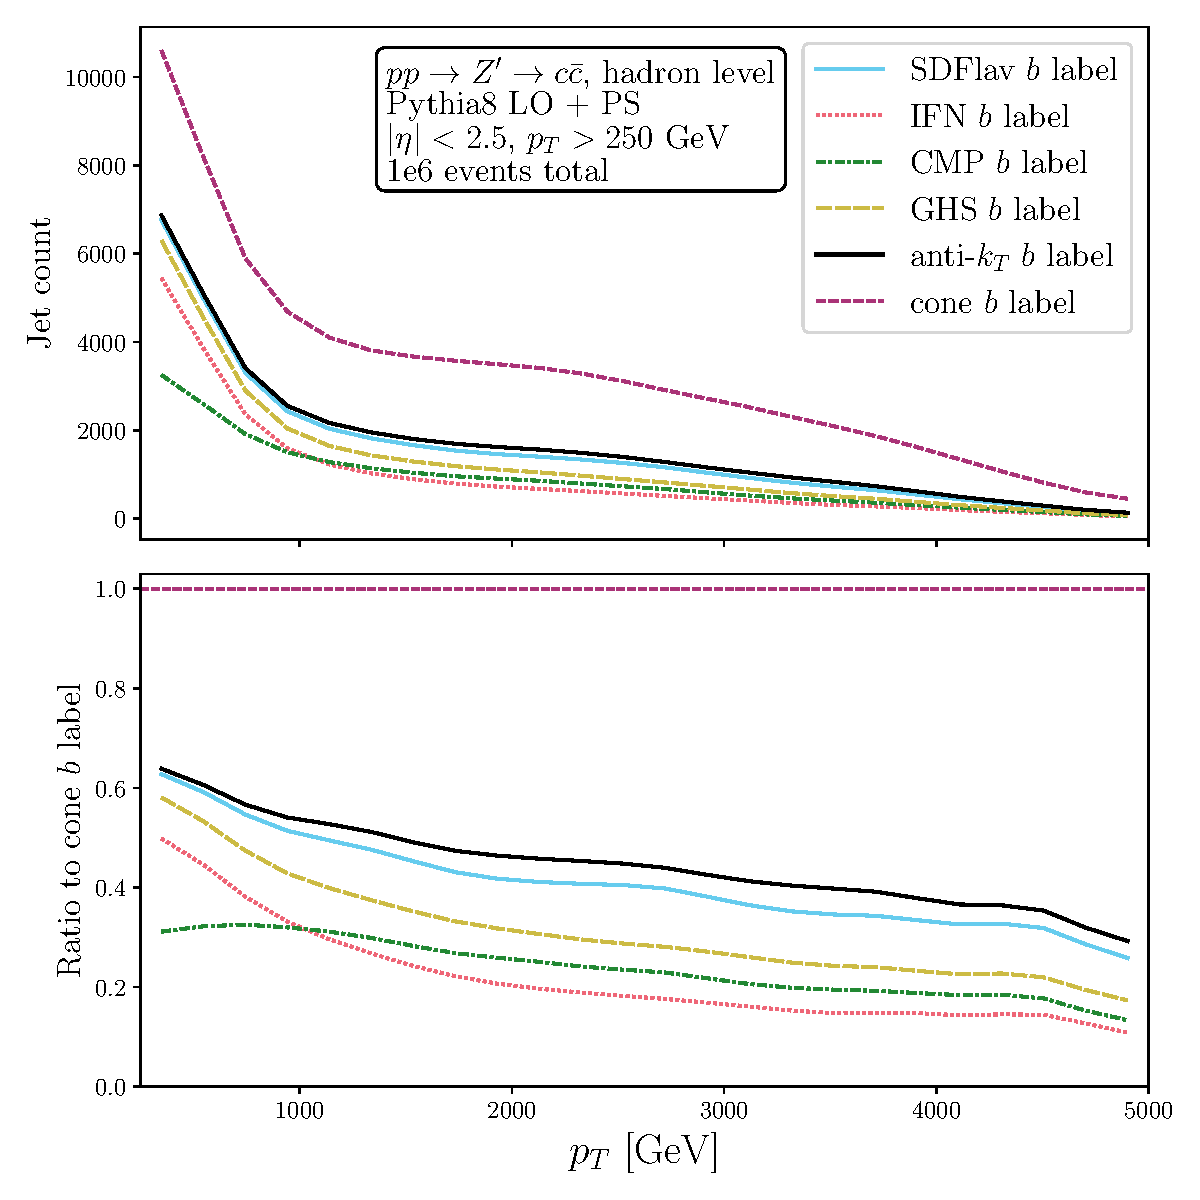
\includegraphics[width=0.49\linewidth]{ftag/NETno-grey-line-BLACKANTIKT-MAINCBFN-CMP-ATLAS-compare-pt-with-ratio}}\\
    \subfloat[\label{b_or_c}]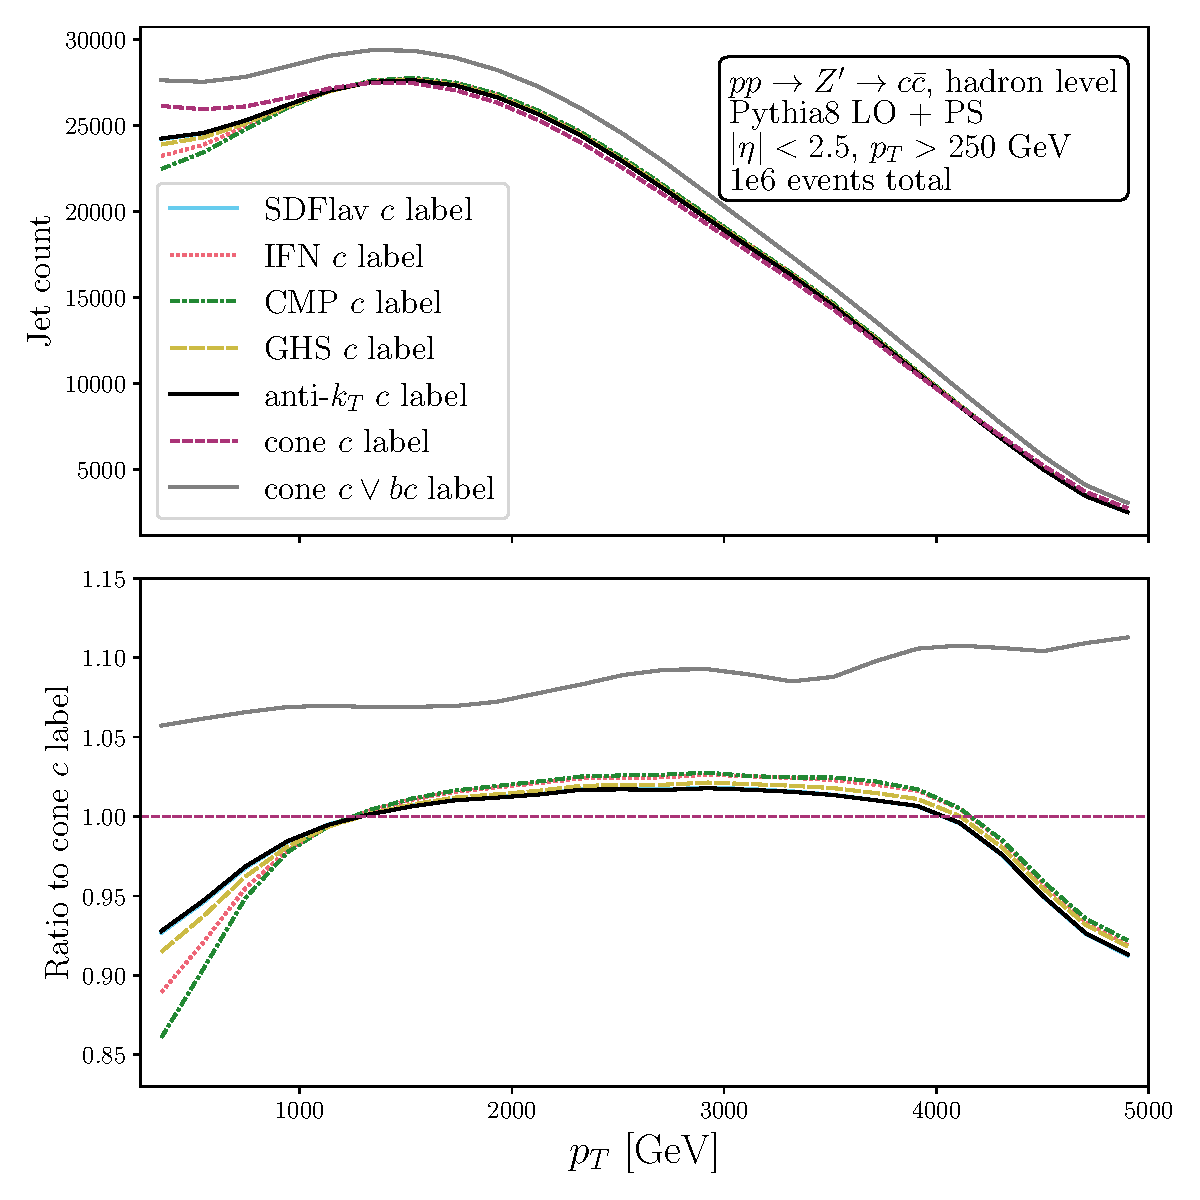
\includegraphics[width=0.49\linewidth]{ftag/NETBLACKANTIKT-MAINCIFN-CMP-ATLAS-compare-pt-with-ratio.pdf}
    
    \caption{The $p_t$ spectra of $c$ jets (top left) and $b$ jets (top right) found in $pp \rightarrow Z\prime \rightarrow c \bar{c}$ events, and the same $p_t$ spectrum including jets containing both $b$ and $c$ jets as identified by the cone algorithm (bottom)~\cite{Behring:2025ilo}.}
    \label{fig:ATLAS-FTAG-comparison}
\end{figure}

This again highlights a shortcoming in flavour labelling used by the ATLAS collaboration. It is necessary to take into account multiple labels when developing a training sample to avoid misidentifying hard $c$-jets as $b$-jets. In these cases, the label assigned is wrong even if one is purely interested in fragmentation studies, as these are jets where the $p_t$ of the $c$-quark can be far greater than than that of the $b$-quark arising from the splitting. 

\subsection{Jet substructure}

Finally, we investigate the effects of flavour labelling on jet substructure, specifically concentrating on the Lund Jet Plane and the jet angularities. 

The investigation of the Lund Jet Plane was carried out as part of the study described in Section~\ref{eo constituents}. The aim was to understand if, correcting for the effect of jet constituents, there were significant differences in the substructure found by the algorithms and the current experimental labelling strategies (ghost). To account for the difference in the constituents, only jets with undecayed heavy hadrons were considered.

Figure~\ref{GHOST-IFN lp} shows the ratio of the Lund Jet Planes for jets labelled according to the IFN algorithm and the ghost algorithm. In the principle part of the plane, there are no significant differences for $b$-jets, and slight differences of the order of a few percent for $c$-jets at high $k_t$.  In less populated regions of the plane, jets labelled with ghost are characterised by more emissions, up to over 10\% in the region of the plane populated by wide-angle, hard emissions. 

\begin{figure}
    \centering
    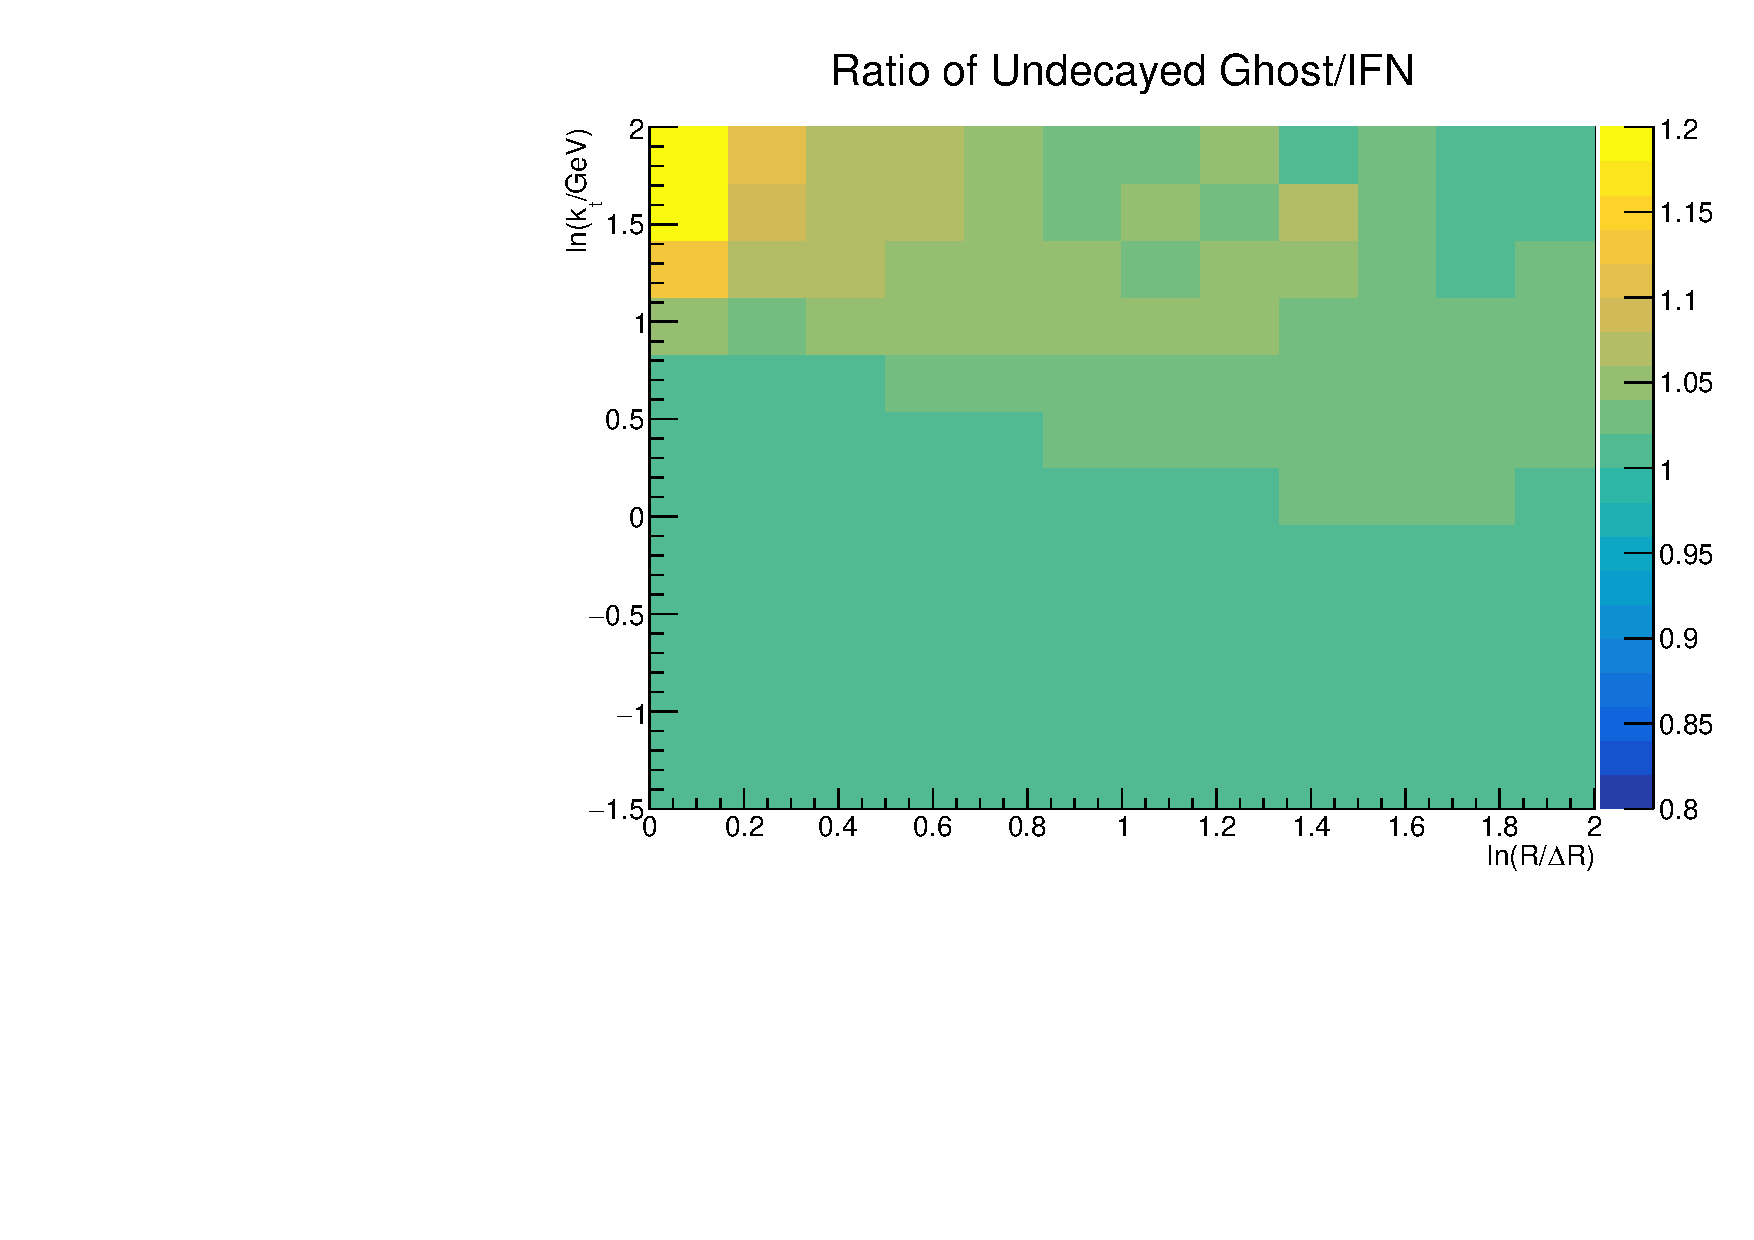
\includegraphics[scale=0.49]{ftag/lpr_b_ghost_undecayed.pdf} 
    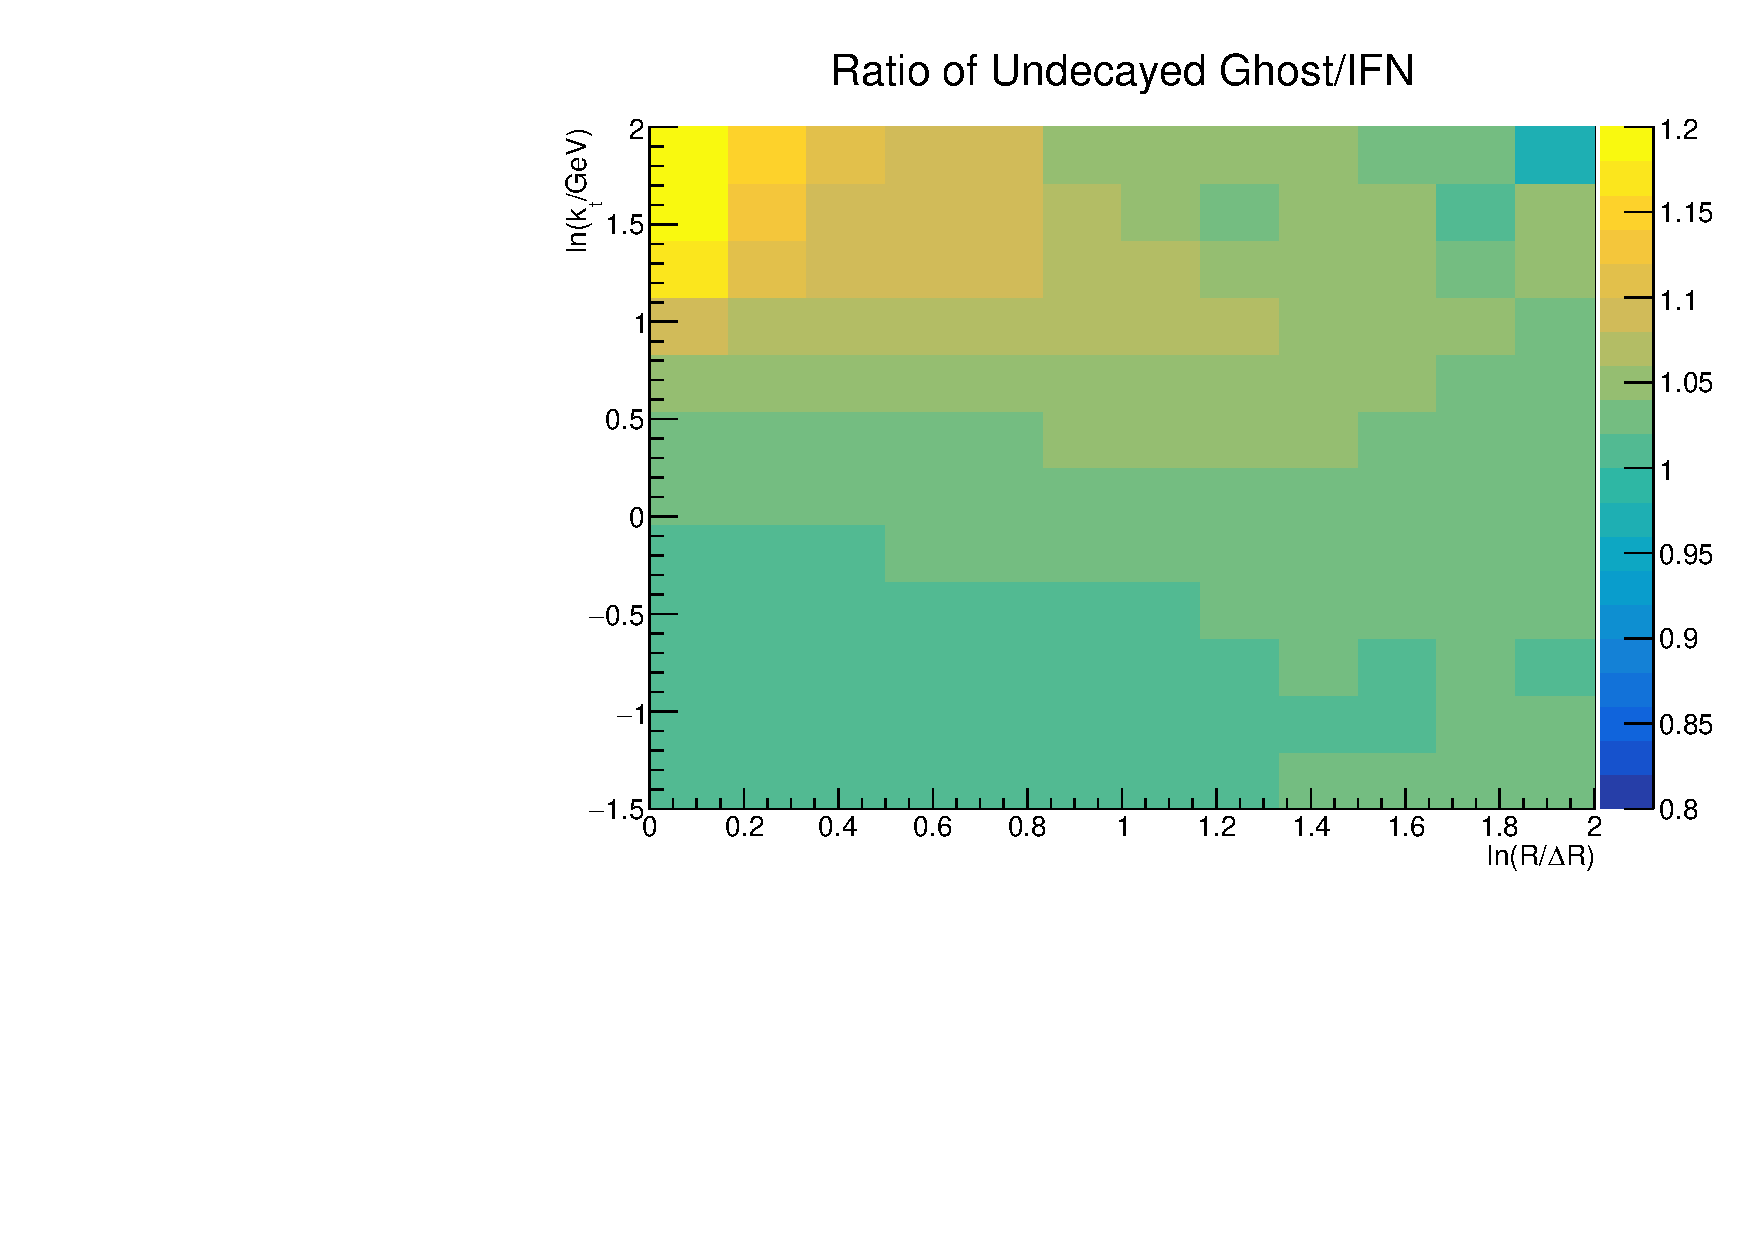
\includegraphics[scale=0.49]{ftag/lpr_c_ghost_undecayed.pdf}
    \caption{The ratio of the Lund Jet Plane for leading $b/c$-jets (left/right) identified with ghost labelling containing undecayed $b/c$ hadrons and those identified with IFN.}
    \label{GHOST-IFN lp}
\end{figure}

In Figure~\ref{fig:nlops_ppzjet_jss_ang}, we show the jet angularities spectrum predicted as part of the study carried out in Section~\ref{flav recomb}. The MC generation was carried out at NLO+PS without hadronisation, and sensitivity to the heavy flavour quark mass is investigated by setting it to zero. Angularities with $\alpha = 0.5$ are shown for $b$-jets and $c$-jets. In the top panel, the differential cross section for the angularities for Sherpa, the Herwig7 angular ordered shower with quark mass, and the Herwig7 dipole shower without quark masses is shown for anti-$k_t$ labelled jets with the mod-2 recombination scheme. The ratio of the flavoured jets, again with the mod-2 recombination scheme, is then shown to the anti-$k_t$ labelled jets for the three parton showers. 

The predictions obtained with the Sherpa and Herwig7 angular ordered showers agree with each other, and the distribution of the angularities is found to be shifted towards larger values compared to the predictions obtained with the massless splitting functions. Small differences are seen between the various flavoured jets algorithms, but these are enhanced when considering $c$-jets. The excess of jets labelled with the ghost algorithm is consistent with wide-angle radiation entering the jet. No differences are observed between the spectrum predicted by the algorithms for $b$-jets and $c$-jets when the massless dipole shower is considered.  
\begin{figure}
    \centering
    \includegraphics[width=0.5\linewidth,page=16]{ftag/ppzj_bottom_nlops_comparisons_appendix.pdf}%
    \includegraphics[width=0.5\linewidth,page=16]{ftag/ppzj_charm_nlops_comparisons_appendix.pdf}
    \caption{The Les Houches angularity $A_{\alpha = 0.5}$ of the leading $b$-jet (left) and $c$-jet (right) for NLO+PS predictions obtained at parton level with massive Sherpa and Herwig7 angular ordered showers and for a massless Herwig7 dipole shower~\cite{Behring:2025ilo}.}
    \label{fig:nlops_ppzjet_jss_ang}
\end{figure}

\end{document}